\documentclass{masterthesis}

\usepackage{hyperref} % links
\usepackage{graphicx}
\usepackage{amsmath}
\usepackage{amssymb}
\usepackage{qcircuit}
\usepackage{braket}
\usepackage{float}
\usepackage[toc,page]{appendix}
\usepackage{tikz}
\usepackage{xcolor}
\usepackage{listings}

\definecolor{listinggray}{gray}{0.9}
\definecolor{lbcolor}{rgb}{0.9,0.9,0.9}
\lstloadlanguages{Python}

\lstset{
    basicstyle=\ttfamily\small,
    language=Python,
    %backgroundcolor=\color{lbcolor},
    frame=single,
    commentstyle=\color[rgb]{0.133,0.545,0.133},
    keywordstyle=\color[rgb]{0,0,1},
    stringstyle=\color[rgb]{0.627,0.126,0.941},
    showtabs=false,
    showspaces=false,
    showstringspaces=false,
    columns=fullflexible,
    mathescape=true,
    breaklines=true,
    keepspaces,
    upquote=true,
    morekeywords={nonlocal,assert,yield,True,False,bytes,None,with,as}, % technically, bytes is not a keyword, but...
    deletekeywords={file,eval},
    moredelim=[is][\color{red}]{`}{`},%
    moredelim=[is][\color{red}]{~red~}{~red~},%
    moredelim=[is][\color{green}]{~green~}{~green~},%
    moredelim=[is][\color{cyan}]{~cyan~}{~cyan~},%
    moredelim=[is][\color{gray}]{~gray~}{~gray~},%
    moredelim=[is][\color{blue}]{~blue~}{~blue~},%
    moredelim=[is][\color{blue}\bfseries]{/*blue*/}{/*blue*/},
    moredelim=[is][\color{red}\bfseries]{/*red*/}{/*red*/},
    moredelim=[is][\color{cyan}\bfseries]{/*cyan*/}{/*cyan*/},
    moredelim=[is][\bfseries]{/*bf*/}{/*bf*/},
    moredelim=[is][]{/***}{***/}
}

\begin{document}

\title{Mathematical Modeling of Quantum Repeaters Chains}

\author{Lorenzo La Corte}

\advisor{}

\examiner{}

\maketitle

\chapter*{Mathematical Model for \\ Waiting Time and Fidelity}

We derive expressions for the waiting time and fidelity of the first generated end-to-end link in the repeater chain protocol. 

First, We derive a recursive definition for the random variable $T_n$, which \textbf{represents the waiting time in a $2n$-segment repeater chain}.

Then, we extend this definition to the Werner parameter $W_n$ of the pair, which stands in one-to-one correspondence to its fidelity $F_n$ using the equation:
\begin{equation}
    F_n = \frac{1 + 3 W_n}{4}.
\end{equation}

The operations we study in the repeater chain protocols, denoted later as \textbf{protocol units}, are
\begin{itemize}
    \item entanglement generation over a single hop,
    \item entanglement distillation,
    \item entanglement swapping.
\end{itemize}

And they all take a duration that is a multiple of ${L_0}/{c}$, the time to send information over a single segment.

For this reason, it is common to denote the waiting time in \textbf{discrete units} of ${L_0}/{c}$, which is a convention we comply with for $T_n$. 

Cutoffs, introduced to optimize quantum repeater protocols, are also expressed in these discrete units.

\newpage
\section*{Heraldeld Entanglement Generation}\label{section:heralded_entanglement_generation}

The first step in the repeater chain protocol is the generation of elementary entanglement between two nodes.
In the following, we derive the waiting time and Werner parameter for the elementary entanglement generation protocol.

\subsection*{Waiting Time for Elementary Entanglement}
In modeling the random variable $T_n$, which represents the waiting time in a $2^n$ segment repeater chain, we can reason by induction.

The base case \textbf{$T_0$ is the waiting time for the generation of elementary entanglement}.

\begin{figure}[ht]
    \centering
    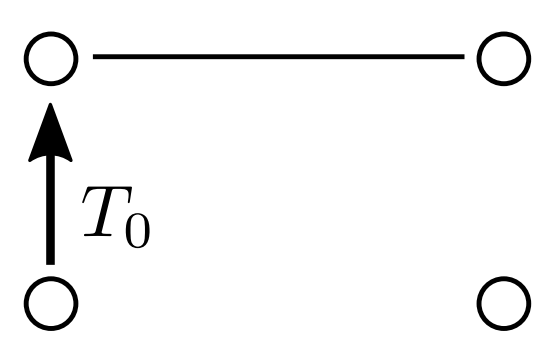
\includegraphics[width=0.2\linewidth]{images/gen.png}
    \caption{For two segments, $T_0$ represents the waiting time for the generation of a single link between two nodes without any intermediate repeater nodes.}
    \label{fig:gen} % todo: add citation
\end{figure}

Since we model the generation of single-hop entanglement by attempts which succeed with a fixed probability $p_{\text{gen}}$, the waiting time $T_0$ is a discrete random variable (in units of $L_0 /c$) which follows a \hyperref[section:geometric_distribution]{geometric distribution} with probability distribution given by 
\begin{equation}
    \Pr(T_0 = t) = p_{\text{gen}} (1 - p_{\text{gen}})^{t-1} \quad \text{for} \quad t \in \{1, 2, 3, \ldots \}
\end{equation}
where $p_{\text{gen}}$ is the probability of success of the entanglement generation protocol.

% tocheck: is it really more convenient to specify T_0 by its CDF? I think in David paper is not like this
% For what follows, it will be more convenient to specify $T_0$ by its \hyperref[subsection:geometric_cdf]{cumulative distribution function} (CDF), which is given by
% \begin{equation}
%     \Pr(T_0 \leq t) = 1 - (1 - p_{\text{gen}})^t.
% \end{equation}

\subsection*{Werner Parameter for Elementary Entanglement}\label{subsection:werner_parameter_gen}

The output state of the entanglement generation protocol is a Werner state with Werner parameter $w_0$.

\subsection*{Numerical Examples}

To plot the CDF and PDF of the waiting time for the entanglement generation protocol, we can use the following code:
\begin{lstlisting}[language=Python]
def entanglement_generation(p_gen=0.5, t_trunc=20):
    parameters = {
        # a protocol is represented by a tuple of 0 and 1,
        # where 0 stands for swap and 1 stands for distillation.
        # this example is a 0-level swap protocol,
        # as we consider only the entanglement generation.
        "protocol": (),
        # success probability of entanglement generation
        "p_gen": p_gen,
        # truncation time for the repeater scheme.
        # It should be increased to cover more time step
        # if the success proability decreases.
        # Commercial hardware can easily handle up to t_trunc=1e5
        "t_trunc": t_trunc
    }
    pmf, _ = repeater_sim(parameters)
    return pmf
\end{lstlisting}
% todo: cite Li_2021
Where the function \texttt{repeater\_sim} is the algorithm introduced in \cite{}, which simulates the repeater chain protocol and returns the probability mass function (PMF) of the waiting time.

The following figures show the CDF and PDF of the waiting time for the entanglement generation protocol, with $p_{\text{gen}} = 0.2$ and $p_{\text{gen}} = 0.5$. We can see that the waiting time is \textbf{distributed according to a geometric distribution}, as expected.

In order for the algorithm to be computationally feasible, \textbf{the waiting time is truncated}, in this case at $t = 20$. 

The parameter $t_{trunc}$ in the algorithm should chosen to be large enough to capture the bulk of the distribution, but small enough to keep the computation time reasonable. 

The truncation brings to an approximation of the distribution, as the probability of waiting for more than 20 units of time is not considered: this is more visible in the top plot, where the CDF is less close to 1 at $t = 20$.

\begin{figure}[ht]
    \centering
    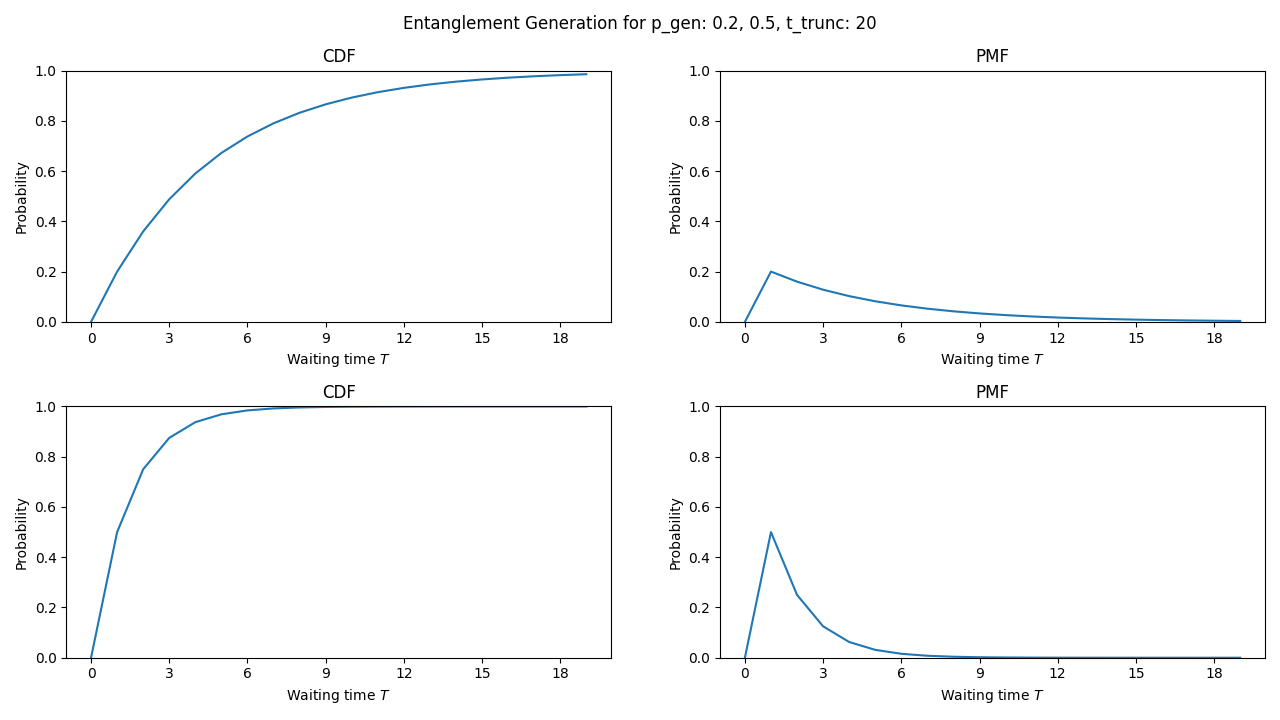
\includegraphics[width=1\linewidth]{images/gen_example_20.png}
    \caption{CDF and PDF of the waiting time for the entanglement generation protocol, with $p_{gen} = 0.2$ (top) and $p_{gen} = 0.5$ (bottom).}
\end{figure}

\newpage
\section*{Entanglement Swapping}

Once we have generated elementary entanglement, we can use it to \textbf{create entanglement over longer distances by entanglement swapping}.

\subsection*{Waiting Time for Entanglement Swapping}

We defined $T_0$ as the waiting time for the generation of elementary entanglement, and our base for the induction.
We now define our inductive step assuming that we have found an expression for $T_n$ and we want to construct $T_{n+1}$. 

In order to perform the entanglement swap to produce a single $(2^n+1)$-hop link, a node needs to wait for the production of two $(2^n)$-hop links, one on each side. 

\begin{figure}[ht]
    \centering
    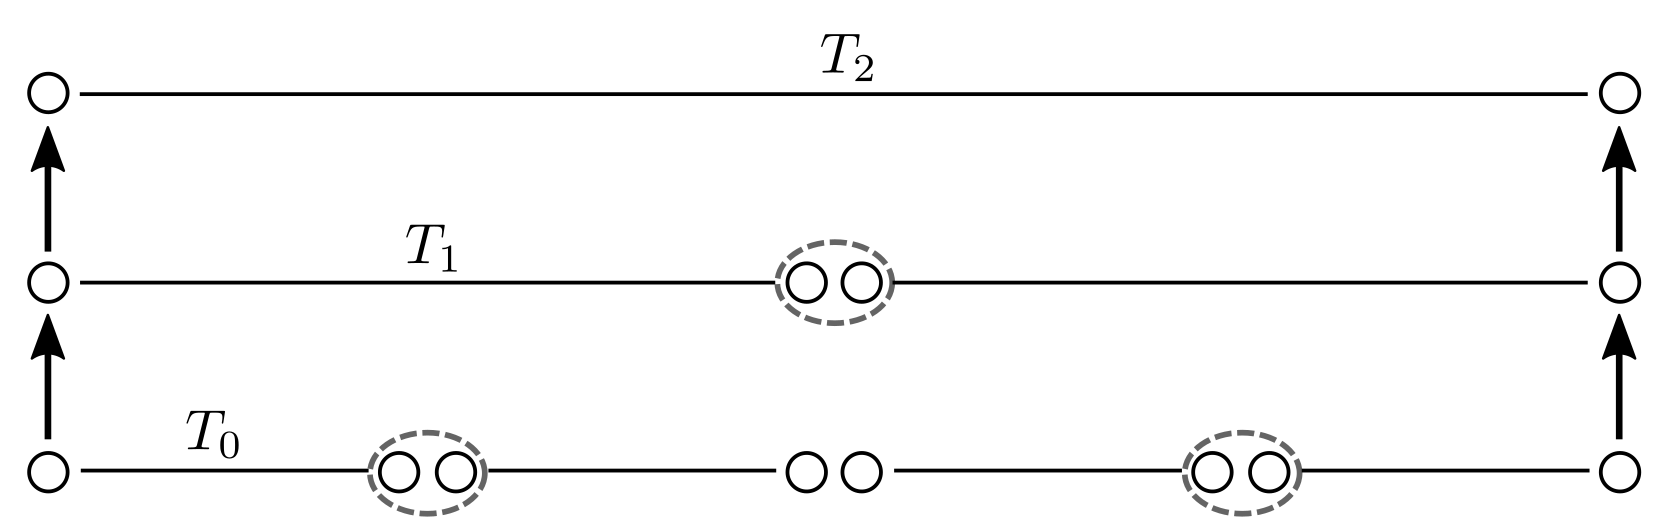
\includegraphics[width=0.8\linewidth]{images/dist.png}
    \caption{A link that spans $2^n$ segments is produced in a nested fashion, where at each nesting level two links are produced and subsequently swapped. \cite{}} % todo: add citation
    \label{fig:dist}
\end{figure}

Denote the waiting time for the pairs by $T_n^{(A)}$ and $T_n^{(B)}$, both of which are i.i.d. with $T_n$, as they are copies of it (see \hyperref[paragraph:copies_of_a_random_variable]{copies of a random variable}).

\subsubsection*{Time until both pairs are available}

We introduce a new random variable $M_n$ modeling the time until both pairs are available
\begin{equation}\label{eq:waiting_time_pair}
    M_n := g_T(T_n^{(A)} , T_n^{(B)}) .
\end{equation}

The function $g_T$ is generally defined as the maximum of the two waiting times
\begin{equation}\label{eq:waiting_time_pair_max}
    g_T(t_A, t_B) := \max(t_A, t_B).
\end{equation}
which is also \textbf{the time at which the entanglement swap ends}. 

This is distributed according to the CDF
\begin{equation}
    \Pr(M_n \leq t) = \Pr(T_n^{(A)} \leq t \text{ and } T_n^{(B)} \leq t) = \Pr(T_n \leq t) ^ 2.
\end{equation}

From it, we can derive the PDF
\begin{align}\label{eq:pdf_waiting_time_pair}
    \Pr(M_n = t) &= \sum_{\substack{t_A, t_B: \\ t = \max(t_A, t_B)}} \Pr(T_n^{(A)} = t_A \text{ and } T_n^{(B)} = t_B) .
\end{align}

% todo: add a concrete example coming from the code, with \Pr(T_n^{(A)} = t_A), \Pr(T_n^{(B)} = t_B and \Pr(M_n = t)

\subsubsection*{Number of steps required}

We introduce now $K_n$, a random variable following a \hyperref[subsection:geometric_pdf]{geometric distribution}
\begin{equation}\label{eq:pdf_swap_steps}
    \Pr(K_n = k) = p_{swap} (1 - p_{swap})^{k-1}
\end{equation}
modeling \textbf{the number of steps $k$ until the first successful swap} at level $n$.

The fact that it follows a geometric distribution is a direct consequence of our choice to model the success probability $p_{swap}$ to be independent of the state of the two input links. 

\subsubsection*{Derivation of $T_{n+1}$}
The derivation of $T_{n+1}$ requires us to combine the random variable for the number of steps required $K_n$ and the random variable for the waiting time for one attempt $M_n$.

In order to find the relation between $M_n$ and $T_{n+1}$, note that when entanglement swap fails, the two input are lost and need to be
regenerated. The regeneration of fresh entanglement after each failing entanglement swap \textbf{adds to the waiting time}. 

Thus, $T_{n+1}$ is a \textit{compound random variable}: it is the sum of $K_n$ copies of $M_n$. 

Since the number of entanglement swaps $K_n$ is geometrically distributed, we say that $T_{n+1}$ is a \textit{geometric compound sum} of $K_n$ copies of $M_n$, denoted as
\begin{equation}
    T_{n+1}=\sum_{k=1}^{K_{n}} M_{n}^{(k)}
\end{equation}

\subsubsection*{Derivation of the PDF of $T_{n+1}$}

The probability distribution of the waiting time $T_{n+1}$
\begin{align}
    \Pr(T_{n+1} = t) &= \Pr\left[\left(\sum_{k=1}^{K_{n}} M_{n}^{(k)}\right) = t\right] \nonumber \\
    \intertext{is computed as the marginal of the waiting time conditioned on a fixed number of swaps}
    \Pr(T_{n+1} = t) &= \sum_{k=1}^{\infty} \Pr(K_{n} = k) \cdot \Pr\left[\left( \sum_{j=1}^{k} M_{n}^{(j)} \right) = t\right].
\end{align}

Plugging in the expressions for $\Pr(K_n = k)$ (Equation \ref{eq:pdf_swap_steps}) and recalling that the sum of $k$ copies of $M_n$ can be expressed as a \hyperref[eq:convolution]{convolution}, we get
\begin{equation}\label{eq:waiting_time_swap}
    \Pr(T_{n+1} = t) = \sum_{k=1}^{\infty} p_{\text{swap}}(1 - p_{\text{swap}})^{k-1} \left( \ast_{j=1}^{k} m \right)
\end{equation}
where, from Equation \ref{eq:pdf_waiting_time_pair}
\begin{equation}\label{eq:pdf_waiting_time_pair_convolution}
    m(t) := \Pr(M = t) = \sum_{\substack{t_A, t_B: \\ t = \max(t_A, t_B)}} \Pr(T_n^{(A)} = t_A \text{ and } T_n^{(B)} = t_B) .
\end{equation}

\subsection*{Werner Parameter for Entanglement Swapping}

Considering two entangled pairs, respectively with Werner parameters $w_A$ and $w_B$, the output Werner parameter $w_{out}$, if we do not consider decoherence, will be % todo: for the thesis, cref werner parameter
\begin{equation}
    w_{out} = w_A \cdot w_B .
\end{equation}

However, when the first of the two pairs is generated, it has to wait for the elementary generation of the other; \textbf{during this time the first generated pair decoheres}. In particular, a Werner state $\rho(w)$ residing in memory for a time $\Delta(t)$ will transform into the Werner state $\rho(w_{decayed})$ with 
\begin{equation}\label{eq:w_decayed}
    w_{\text{decayed}} = w \cdot e^{-\Delta t / T_{coh}}
\end{equation}
where $T_{coh}$ is the joint coherence time of the two quantum memories holding the qubits. % todo: for the thesis, refer to coherence time and q. memories

Denote by $A$ and $B$ the input links to the entanglement swap and denote by $\left(t_{A}, w_{A}\right)$ and $\left(t_{B}, w_{B}\right)$ their respective delivery times and Werner parameters. 
% todo: add image
Without loss of generality, suppose that the link $A$ is produced after link $B$, i.e. $t_{A} \geq t_{B}$. 

Link $A$ is produced last, so the entanglement swap will be performed directly after its generation and hence link $A$ will enter the entanglement swap with Werner parameter $w_{A}$. Link $B$ is produced earliest and will therefore decohere until production of link $A$.

It follows that $B$'s Werner parameter decoheres accordingly to (\ref{eq:w_decayed}), and therefore is, immediately before the swap, equal to
\begin{equation*}
    w_{B}^{\prime} = w_{B} \cdot e^{-\left|t_{A}-t_{B}\right| / T_{coh}} .
\end{equation*}

Thus, the entanglement swap would produce the $2^{n+1}$-hop state with Werner parameter
\begin{align}
w_{out} &= w_{A} \cdot w_{B}^{\prime} \nonumber \\
        &= w_{A} \cdot w_{B} \cdot e^{-\left|t_{A}-t_{B}\right| / T_{coh}} .
\end{align}

Notice that choosing $t_{A} > t_{B}$ would have lead to the same result.
% todo: include figure 2 of Li paper
In order to model at the same time the Werner Parameter and the Waiting Time we use a joint random variable $(T_n, W_n)$.

In the \textbf{base case}, for a single segment ($n=0$), we are in the \hyperref[subsection:werner_parameter_gen]{(already discussed)} entanglement generation phase.
Here, the \textbf{waiting time and Werner parameter are uncorrelated} because we model the attempts at generating single-hop entanglement to be independent and to each take equally long. 

At the \textbf{recursive step} $n$, we model the waiting time and Werner parameter as a joint random variable $(T_n, W_n)$.

\paragraph*{Forgetting Sum} To define it properly, we introduce the concept of \textit{forgetting sum} $\widehat{\sum}$, defined on sequences of tuples $\left\{\left(x_{j}, y_{j}\right) \mid 1 \leq j \leq m\right\}$ for some $m \in\{1,2, \ldots\}$ as
\begin{equation}\label{eq:forgetting_sum}
    \widehat{\sum}_{j=1}^{m}\left(x_{j}, y_{j}\right):=\left(\sum_{j=1}^{m} x_{j}, y_{m}\right)
\end{equation}

This notation is key to characterize the joint random variable $(T_{n+1}, W_{n+1})$, as the Werner parameter of the output link is only influenced by the links that the successful entanglement swap acted upon, as we will see in the following.

Using this concept, we define the joint random variable $(T_{n+1}, W_{n+1})$ as
\begin{equation}\label{eq:joint_random_variable}
    (T_{n+1}, W_{n+1}) := \widehat{\sum}_{k=1}^{K_n} (M_n, V_n)^{(k)}.
\end{equation}

Starting from the auxiliary variable for the output waiting time of a pair $M_n$ (Eq. \ref{eq:waiting_time_pair}), we introduce another auxiliary random variable for the Werner parameter of the output link $V_n$, which will depend on the Werner parameters of the input links. 

We define the auxiliary joint random variable $(M_n, V_n)$ as
\begin{equation}
    (M_n, V_n) := g\left((T_n, W_n)^{(A)}, (T_n, W_n)^{(B)}\right).
\end{equation}

The function $g$ is given by
\begin{equation}
    g\left((t_A, w_A),(t_B, w_B)\right) := \left(g_T(t_A, t_B), g_W\left((t_A, w_A),(t_B, w_B)\right)\right)
\end{equation}
where $g_T$ is defined in Eq. \ref{eq:waiting_time_pair_max} and
\begin{equation}
    g_W\left((t_A, w_A),(t_B, w_B)\right) := w_A \cdot w_B \cdot e^{-\left|t_{A}-t_{B}\right| / T_{coh}} .
\end{equation}
with $T_{\text{coh}}$ the quantum memory coherence time.

We already studied the expression for the waiting time $T_{n+1}$. The other random variable $W_{n+1}$ directly derives from $V_{n}$, which expresses the Werner parameter of the produced $2^{n+1}$-hop link in case the swap is successful.

To prove that $V_{n}$ is formulated properly, we argue that $g_{W}$ correctly computes the Werner parameter of the output link after an entanglement swap.

The key idea that leads to the forgetting sum in Equation \ref{eq:joint_random_variable} is the following: if the entanglement swap fails, then the $2^{n+1}$-hop link with its Werner parameter will never be produced since both initial $2^{n}$-hop entangled pairs are lost. Thus, \textbf{for the waiting time we should consider the sum of the waiting times of all the attempts, but for the Werner parameter we should only consider the last successful attempt}.

Let's explain it further.

In order to find how the Werner parameter on level $n+1$ is expressed as a function of the waiting times and Werner parameters at level $n$, consider a sequence $\left(m_{j}, v_{j}\right)$ of waiting times $m_{j}$ and Werner parameters $v_{j}$, where $j$ runs from 1 to the first successful swap $k$. 
\begin{itemize}
    \item $m_{j}$ correspond to the waiting time until the end of the entanglement swap that transforms two $2^{n}$-hop links into a single $2^{n+1}$-hop link
    \item $v_{j}$ to the output link's Werner parameter if the swap were successful. 
\end{itemize}

From previous results, we found that the total waiting time is given by $\sum_{j=1}^{k} m_{j}$, the sum of the \begin{equation*}
    \begin{array}{|c|c|c|c|}
        \hline
        \text{Time Step} & \text{PMF} & \text{CDF} & \text{Werner} \\
        \hline
        t = 1 & 0.50000 & 0.50000 & 0.90000 \\
        \hline
        t = 2 & 0.25000 & 0.75000 & 0.90000 \\
        \hline
        t = 3 & 0.12500 & 0.87500 & 0.90000 \\
        \hline
        t = 10 & 0.00098 & 0.99902 & 0.90000 \\
        \hline
        t = 50 & 0.00000 & 1.00000 & 0.90000 \\
        \hline
    \end{array}
\end{equation*}successful one, the output link is the last produced link and therefore its Werner parameter equals $v_{k}$. 

We thus find that the waiting time $t_{\text {final }}$ of the first $2^{n+1}$-hop link and its Werner parameter $w_{\text {final }}$ are given by:
\begin{align}
    t_{final} &= \sum_{j=1}^{k} m_{j} \\ 
    w_{final} &= v_k 
\end{align}
or, in a more compact form
\begin{equation}
    \left(t_{final}, w_{final}\right) = \left(\sum_{j=1}^{k} m_{j}, v_{k}\right) .
\end{equation}

Taking into account that the number of swaps $k$ that need to be performed until the first successful one is an instance of the random variable $K_{n}$, we arrive at the full recursive expression for the waiting time and Werner parameter at level $n+1$ as given in Equation \ref{eq:joint_random_variable}.

\subsubsection*{Derivation of $W_{out}$}
Let's now derive the expression for the Werner parameter of the output link $W_{out}$.

Let $W_{s}(t)$ be the \textbf{average Werner parameter} of the output link of \textbf{one attempt}, given that it succeeds and finishes at time $t$
\begin{equation}
    W_s(t) = \sum_{\substack{t_A, t_B:\\ t = \max(t_A, t_B)}} \Pr(T_A = t_A, T_B = t_B) \cdot [p_{swap} \cdot w_{\text{out}}](t_A, t_B)
\end{equation}

By taking Eq. \ref{eq:joint_random_variable} and replacing the iteration over all pair of possible input Werner parameters for each $k$ by convolution we get
\begin{equation}\label{werner_parameter_swap}
    W_{out} = \sum_{k=1}^{\infty} p_{swap} (1 - p_{swap})^{k-1} \left[ \left( \ast_{j=1}^{k-1} m \right) \ast \left( m \cdot W_{s} \right) \right]
\end{equation}
where $m$ is defined in Eq. \ref{eq:pdf_waiting_time_pair_convolution}.

$W_{out}$ represents the weighted average of the Werner parameter of the output link, over all possible sequences of failed attempts, followed by a successful one:
\begin{itemize}
    \item all possible sequences of failed attempts are represented by the $k-1$ of $m$,
    \item the successful attempt is represented by the convolution of $m$ and $W_{s}$.
\end{itemize}

\subsection*{Numerical Examples}

To plot CDF, PDF and Werner parameter of the waiting time for a 3-level entanglement swapping protocol, we can use the following code snippet:
\begin{lstlisting}[language=Python]
    def entanglement_swap(p_gen=0.5, p_swap=0.5, w_0=0.99, t_trunc=20):
        parameters = {
            # 3-level swap protocol, without distillation
            # spanning over 9 nodes (8 segments)
            "protocol": (0, 0, 0),
            "p_gen": p_gen,
            "p_swap": p_swap,
            "t_trunc": t_trunc,
            "w0": w_0,
            # the memory coherence time 
            # in the unit of one attempt of elementary link generation
            "t_coh": 400,
        }
        pmf, w_func = repeater_sim(parameters)
        
        # remove unstable Werner parameter
        t = 0
        while(pmf[t] < 1.0e-17):
            w_func[t] = np.nan
            t += 1

        return pmf, w_func
\end{lstlisting}

The Figure \ref{fig:swap} shows the CDF and PDF of the waiting time for the entanglement swapping protocol, with $p_{gen} = 0.2$, $p_{swap} = 0.2$, and $t_{trunc} = 8000$. 

The truncation approximated the distribution: the probability of waiting for more than 200 units of time is not considered. Thus, the plot only covers 98.57\% of the distribution. However, the initial bit of the Werner parameter curve is more visible using this truncation.

We can see that the Werner parameter, which measures the quality of the entanglement
\begin{itemize}
    \item starts from a value around $0.43$,
    \item immediately, at $t = 8$, reaches its peak value of $0.87$,
    \item rapidly decreases, reaching a value similar to the starting one.
\end{itemize}

This is due to the fact that the entanglement is lost over time, and the longer the waiting time, the lower the quality of the entanglement.
% todo: but this doesn't explain why in the first few instant it is so low
\begin{figure}[ht]
    \centering
    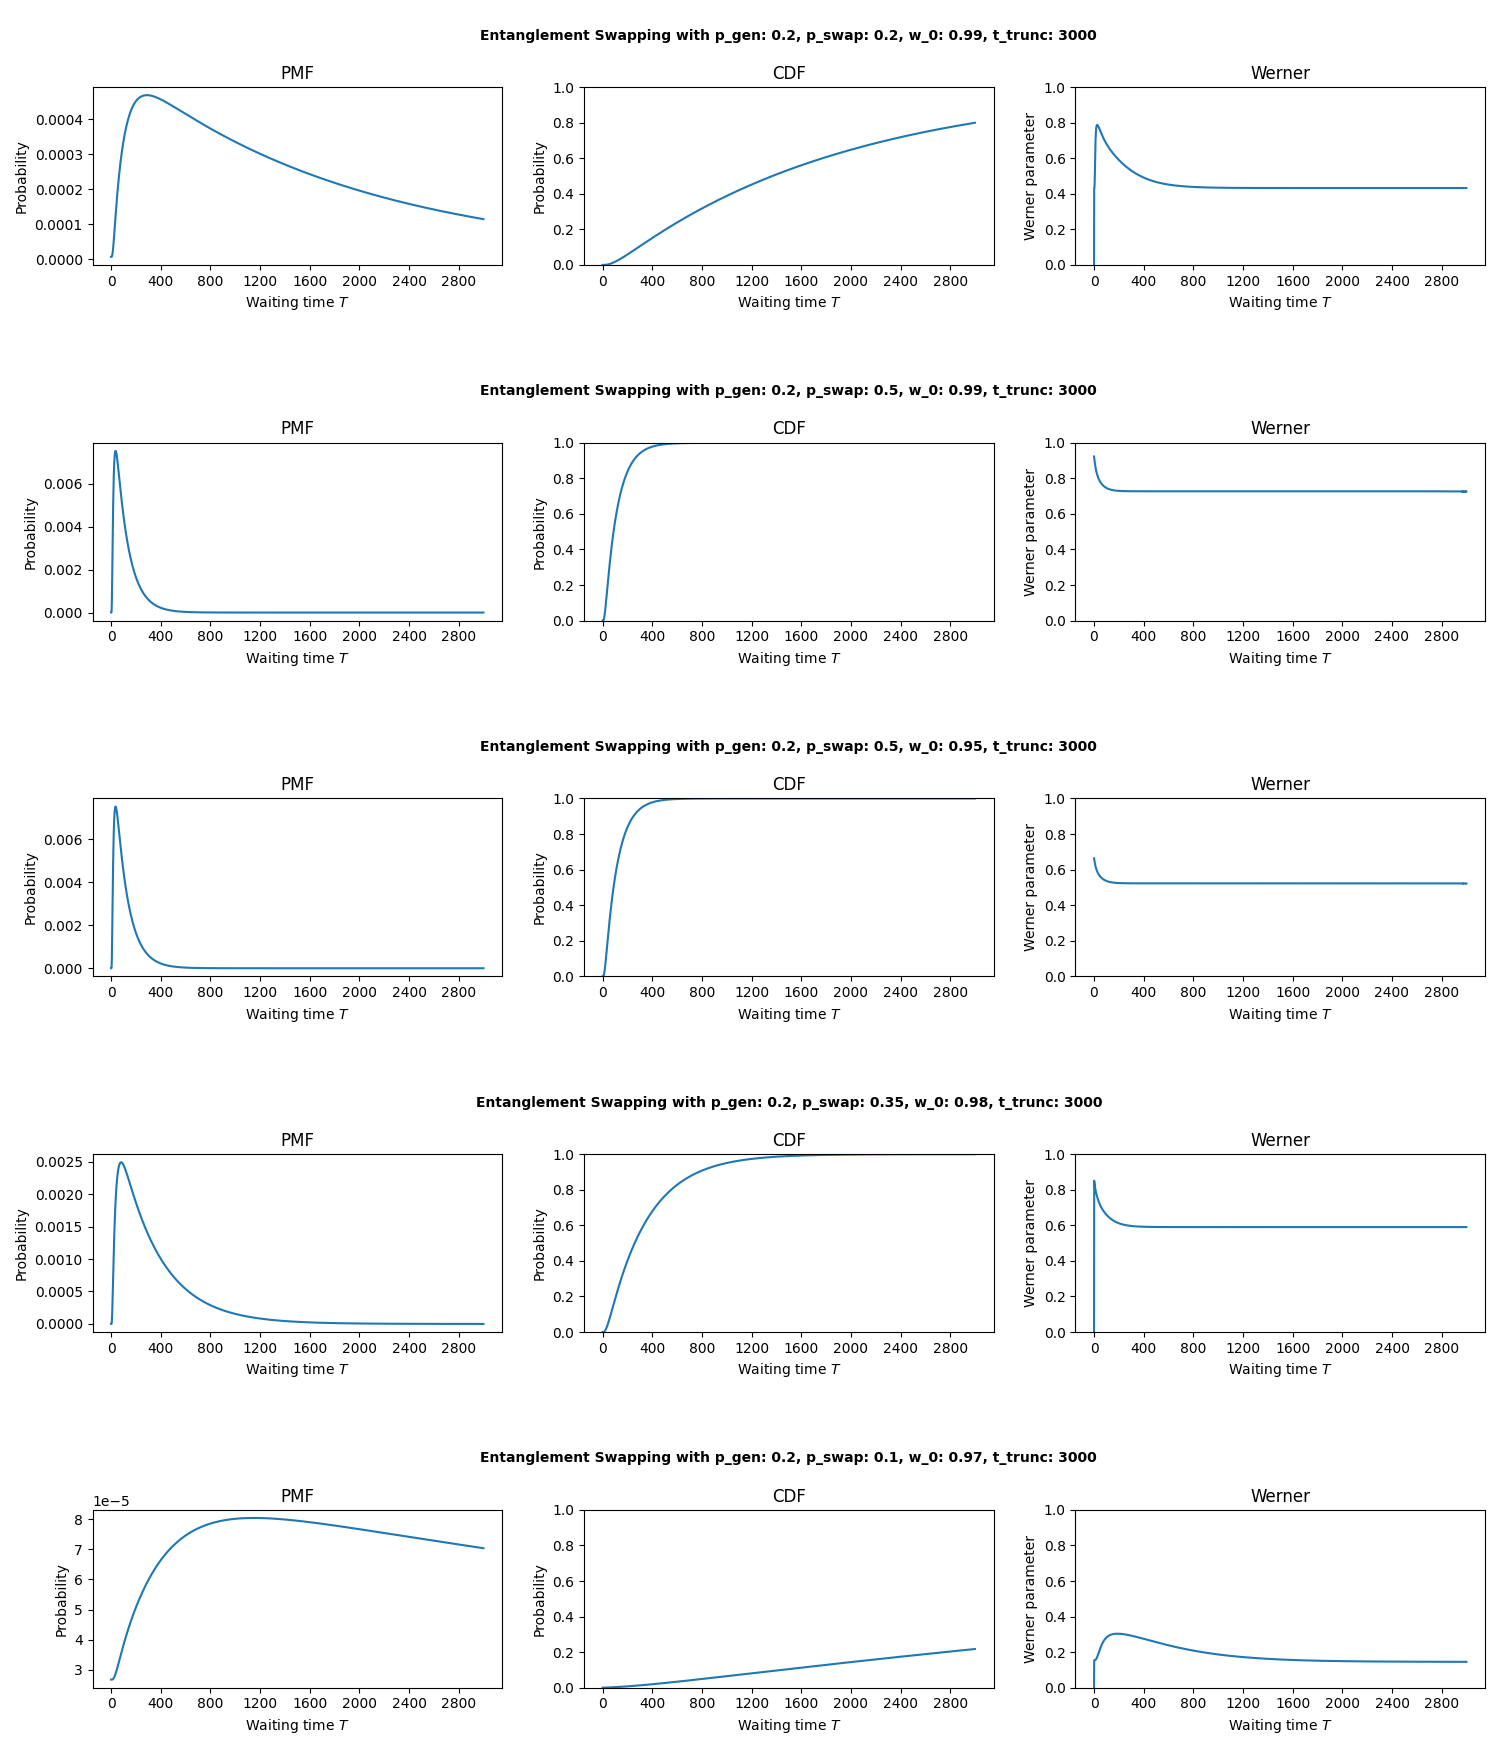
\includegraphics[width=1\linewidth]{images/swap_example_3000.png}
    \caption{CDF and PDF of the waiting time for the entanglement swapping protocol, with $p_{gen} = 0.2$, $p_{swap} = 0.2$, $w_0 = 0.99$ and $t_{trunc} = 8000$.}
    \label{fig:swap}
\end{figure}

We can also compare the undament of the three curves using two different input Werner parameters, as showed in Figure \ref{fig:swap_comparison}.

\begin{figure}[ht]
    \centering
    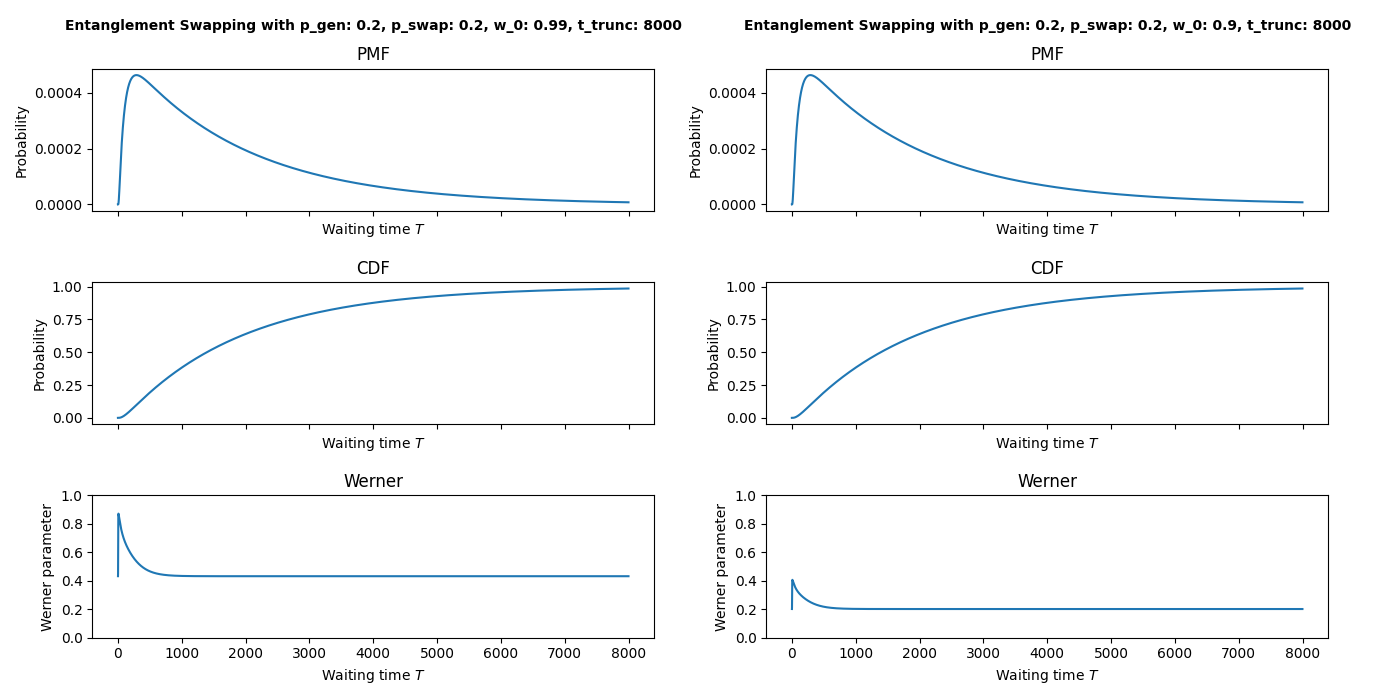
\includegraphics[width=1\linewidth]{images/swap_n3_comparison.png}
    \caption{CDF and PDF of the waiting time for the entanglement swapping protocol, with $p_{gen} = 0.2$, $p_{swap} = 0.2$, $t_{trunc} = 8000$, and $w_0 = 0.99$ (left) and $w_0 = 0.9$ (right).}
    \label{fig:swap_comparison}
\end{figure}

The waiting time distribution is not affected by the initial Werner parameter $w_0$, as expected.

The Werner parameter drops in both the experiments, as already mentioned before.
Notice that the difference between initial qualities of entanglement $w_0 = 0.99$ and $w_0 = 0.9$ impacts heavily on the undament for the Werner parameter.

\newpage
\section*{Entanglement Distillation}

Entanglement distillation takes in input two low-quality entangled pairs and produces a single high-quality one.
% todo: add image
For entanglement distillation, the success probability $p_{dist}$ depends on the Werner parameters of the input links $A$ and $B$; in particular
\begin{equation}
    p_{dist} = \cfrac{1+w_A'w_B'}{2}
\end{equation}
where the primed notation denotes the Werner parameter with decay applied only to the link that waits in memory.

To compute $T_{out}$ and $W_{out}$ for this protocol unit we \textbf{separate the expressions} for the waiting time probability distribution of a successful and failed attempt, respectively $P_s(t)$ and $P_f(t)$.

These are computed by iterating over all possible combinations of the input links' generation time $t_A$, $t_B$ that lead to a waiting time $t$ for this attempt.

We then express the total waiting time distribution $T_{out}$ and the Werner parameter $W_{out}$ as those of the successful attempt averaged by the occurrence probability of all possible sequences of failed attempts, where the weighted average is efficiently computed using convolution (see Equation \ref{eq:convolution}). % todo: for the thesis, reference appendix

\subsection*{Waiting Time for Entanglement Distillation}

To compute he waiting time distribution we consider the generation time of a successful or failed attempt separately and use the joint distribution of $M$ and $Y$, where again $M$ is the waiting time and $Y$ is a binary variable that indicates the success of the attempt. % todo: maybe ref

We define the joint distribution that \textbf{one attempt} succeeds or fails and takes time $t$ as % todo: maybe sep. in two lines the max
\begin{align}\label{eq:waiting_time_success_failure}
    P_s(t) &:= \Pr(M = t, Y = 1) = \sum_{t_A, t_B : t = \max(t_A, t_B) + t_c} \Pr(T_A = t_A, T_B = t_B) \cdot p(t_A, t_B) \\
    P_f(t) &:= \Pr(M = t, Y = 0) = \sum_{t_A, t_B : t = \max(t_A, t_B) + t_c} \Pr(T_A = t_A, T_B = t_B) \cdot [1 - p(t_A, t_B)]
\end{align}
where $t_c$ is the time used for classical communication and local operation. Here, we iterated over all possible combinations of the input links' generation time $t_A$, $t_B$ that leads to a waiting time $t$ for this attempt.

The sum of the waiting time for \textbf{all attempts} can be obtained by
\begin{align}\label{eq:waiting_time_distillation}
    \Pr(T_{out} = t) = \sum_{k=1}^{\infty} \left[ \left( \ast_{j=1}^{k-1} P_f \right) \ast P_s \right]
\end{align}
where the sum over $k$ considers all the possible numbers of attempts, convoluting, for each case, $k-1$ unsuccessful attempts and one successful one.

Neither $P_f$ or $P_s$ characterizes a random variable since they are joint distributions including $Y$, that is to say, $Ps$ and $Pf$ do not sum up to 1. Instead, we have
\begin{equation}
    \sum_t P_s(t) + \sum_t P_f(t) = 1 .
\end{equation}

The convolution here cannot be simply interpreted as a sum of two random variables. Instead, it is the summed waiting time conditioned on the success/failure of each attempt.

To summarize, the full computation goes as follows:
\begin{enumerate}
    \item We compute $P_f$ and $P_s$: the joint distribution that one attempt succeeds or fails and takes time $t$.
    \item Once these are computed, we can compute $T_{out}$ and $W_{out}$ as convolutions of $k-1$ unsuccessful attempts and one successful one, summing over all possible numbers of attempts $k$.
\end{enumerate}

\subsection*{Werner Parameter for Entanglement Distillation}

Also for the Werner parameter, we use the separate expressions for the successful and failed attempts. 

Moreover we use $W(t)$, the average Werner parameter, to reduce the dependence on Werner parameters to the dependence on the waiting time.

First, we compute the average Werner parameter of the output link of \textbf{one attempt}, given that it succeeds and finishes at time $t$
\begin{equation}
    W_s(t) = \frac{\sum_{\substack{t_A, t_B : \\ t = \max(t_A, t_B) + t_c}} \Pr(T_A = t_A, T_B = t_B) \cdot [p_{dist} \cdot w_{\text{out}}](t_A, t_B)}{P_s(t)}.
\end{equation}
where $w_{out}$ is the Werner parameter of the output link if the distillation attempt \textbf{was successful}.

Next, we take a weighted average of $W_s$ over all possible sequences of failed attempts, followed by a single successful attempt:
\begin{equation}\label{eq:werner_parameter_distillation}
    W_{out} = \frac{\sum_{k=1}^{\infty} \left[ \left( \ast_{i=1}^{k-1} P_f^{(j)} \right) \ast (P_s \cdot W_s) \right] (t)}{\Pr(T_{out} = t)}.
\end{equation}

This give us the Werner parameter of the output link.

\paragraph*{An important remark} From the expressions we derived for the waiting time and the Werner parameter, derived by the separate expressions for the successful and failed attempts, we can also derive in an alternative way the expressions for the Werner parameter and the waiting time for entanglement swapping.

In particular, ... % todo: complete


\subsection*{Numerical Examples}

Here, we present the execution of a protocol involving entanglement generation, distillation, and swapping.

This example does not follow the standard number of nodes. As a matter of fact, we have 3 segments (not a power of two) and 4 nodes, including the end parties A and B.

The protocol is visualized in Figure \ref{fig:mixed_protocol_sketch}, and results from the different steps are shown in Figure \ref{fig:mixed_protocol}.

\begin{figure}[ht]
    \centering
    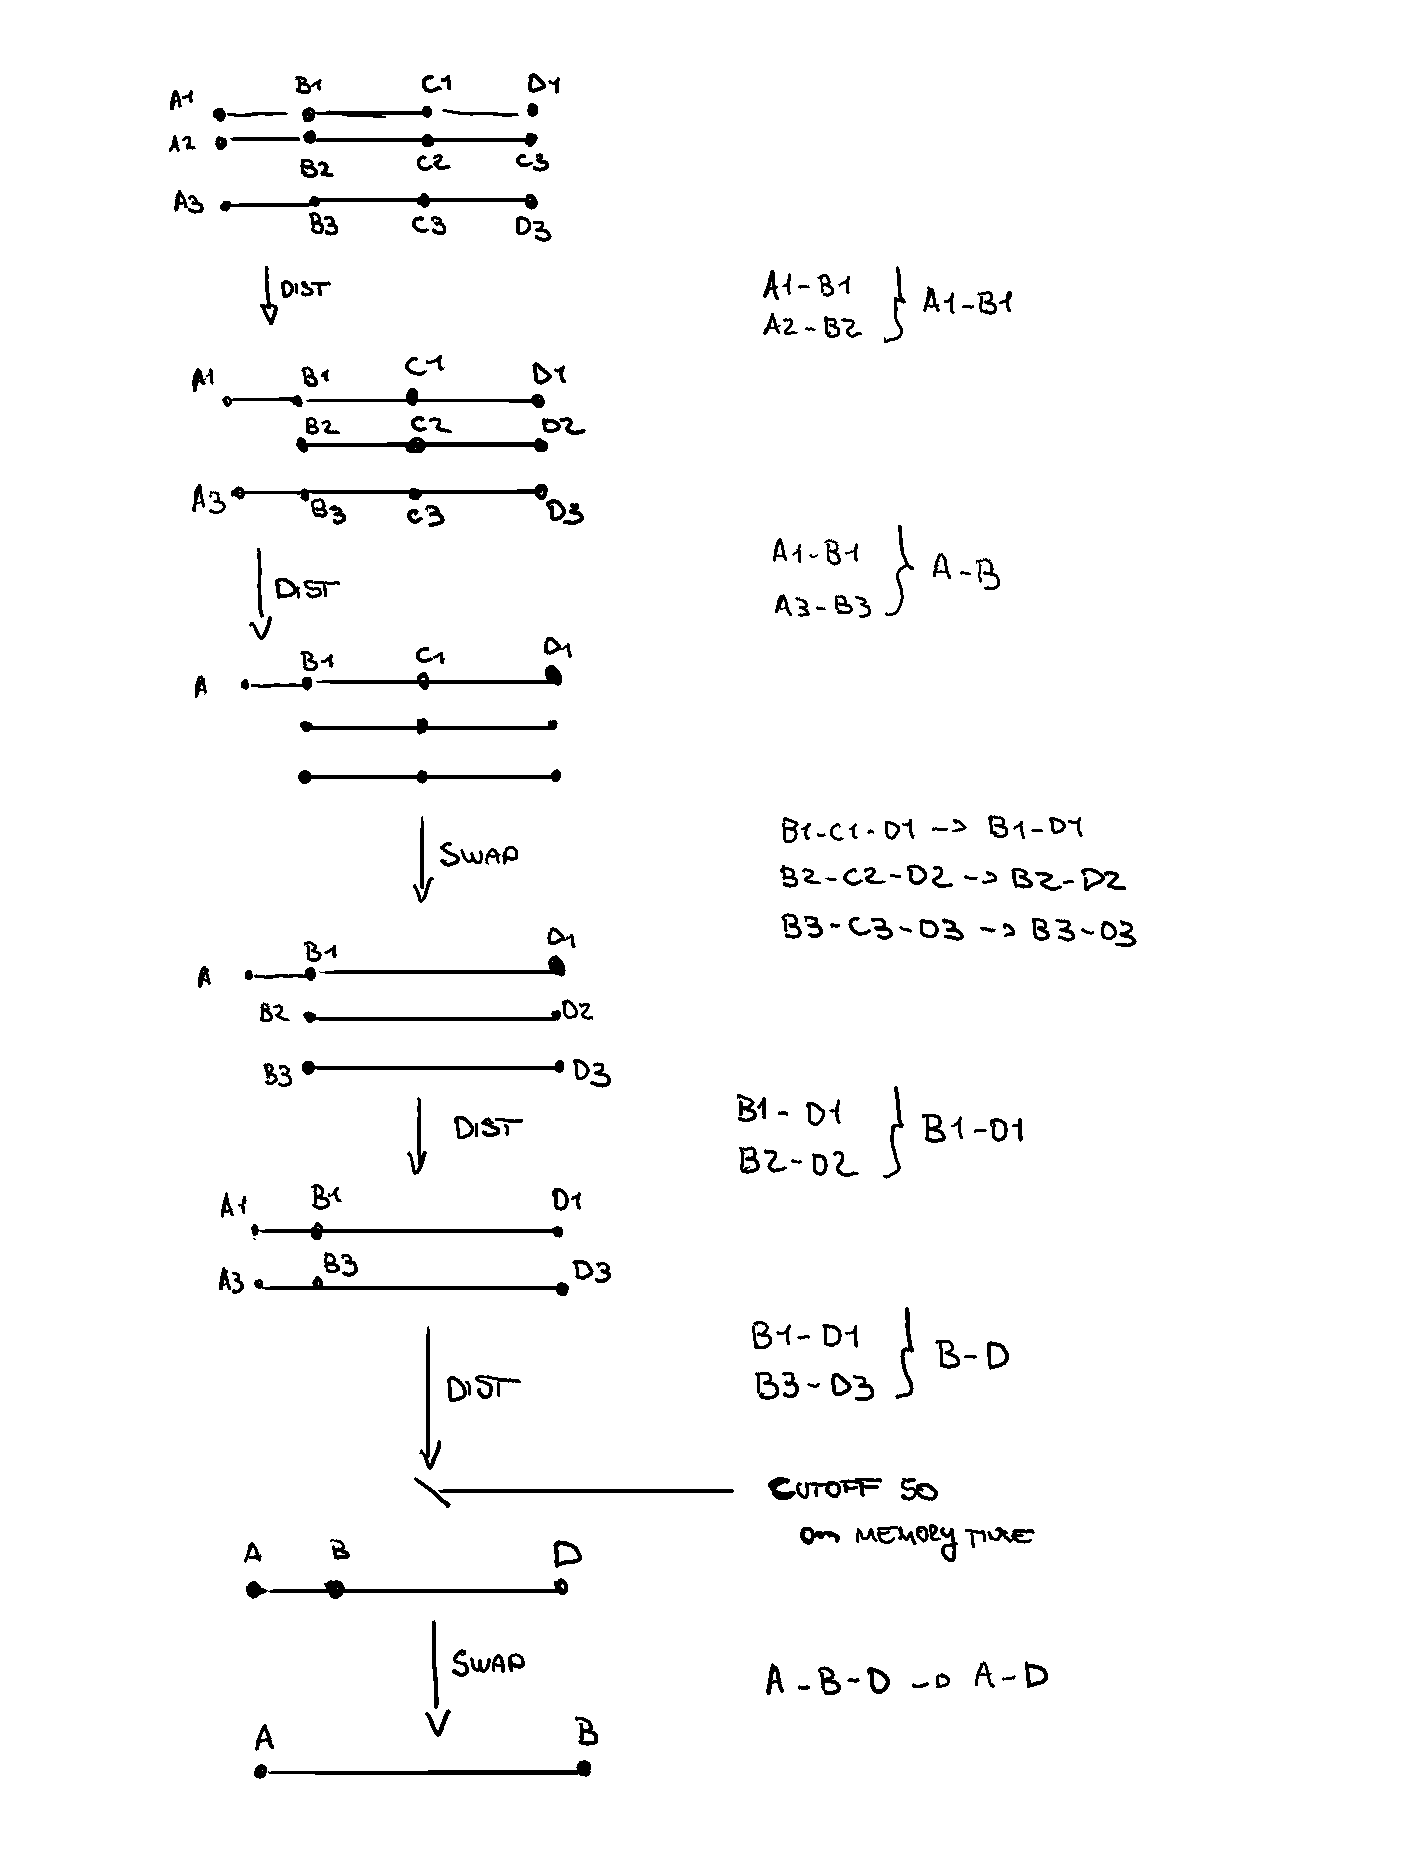
\includegraphics[width=0.8\linewidth]{images/dist_example_sketch.png}
    \caption{We show a mixed protocol, with the number of qubits and segments not being a power of two. Notice that it is only for illustrative purposes, and the protocol is not optimal. We have a four nodes repeater chain with three segments. The end nodes $A$ and $D$ have 3 qubits, while the intermediate nodes $B$ and $C$ have 6 qubits.}
    \label{fig:mixed_protocol_sketch} 
\end{figure}

\begin{figure}[ht]
    \centering
    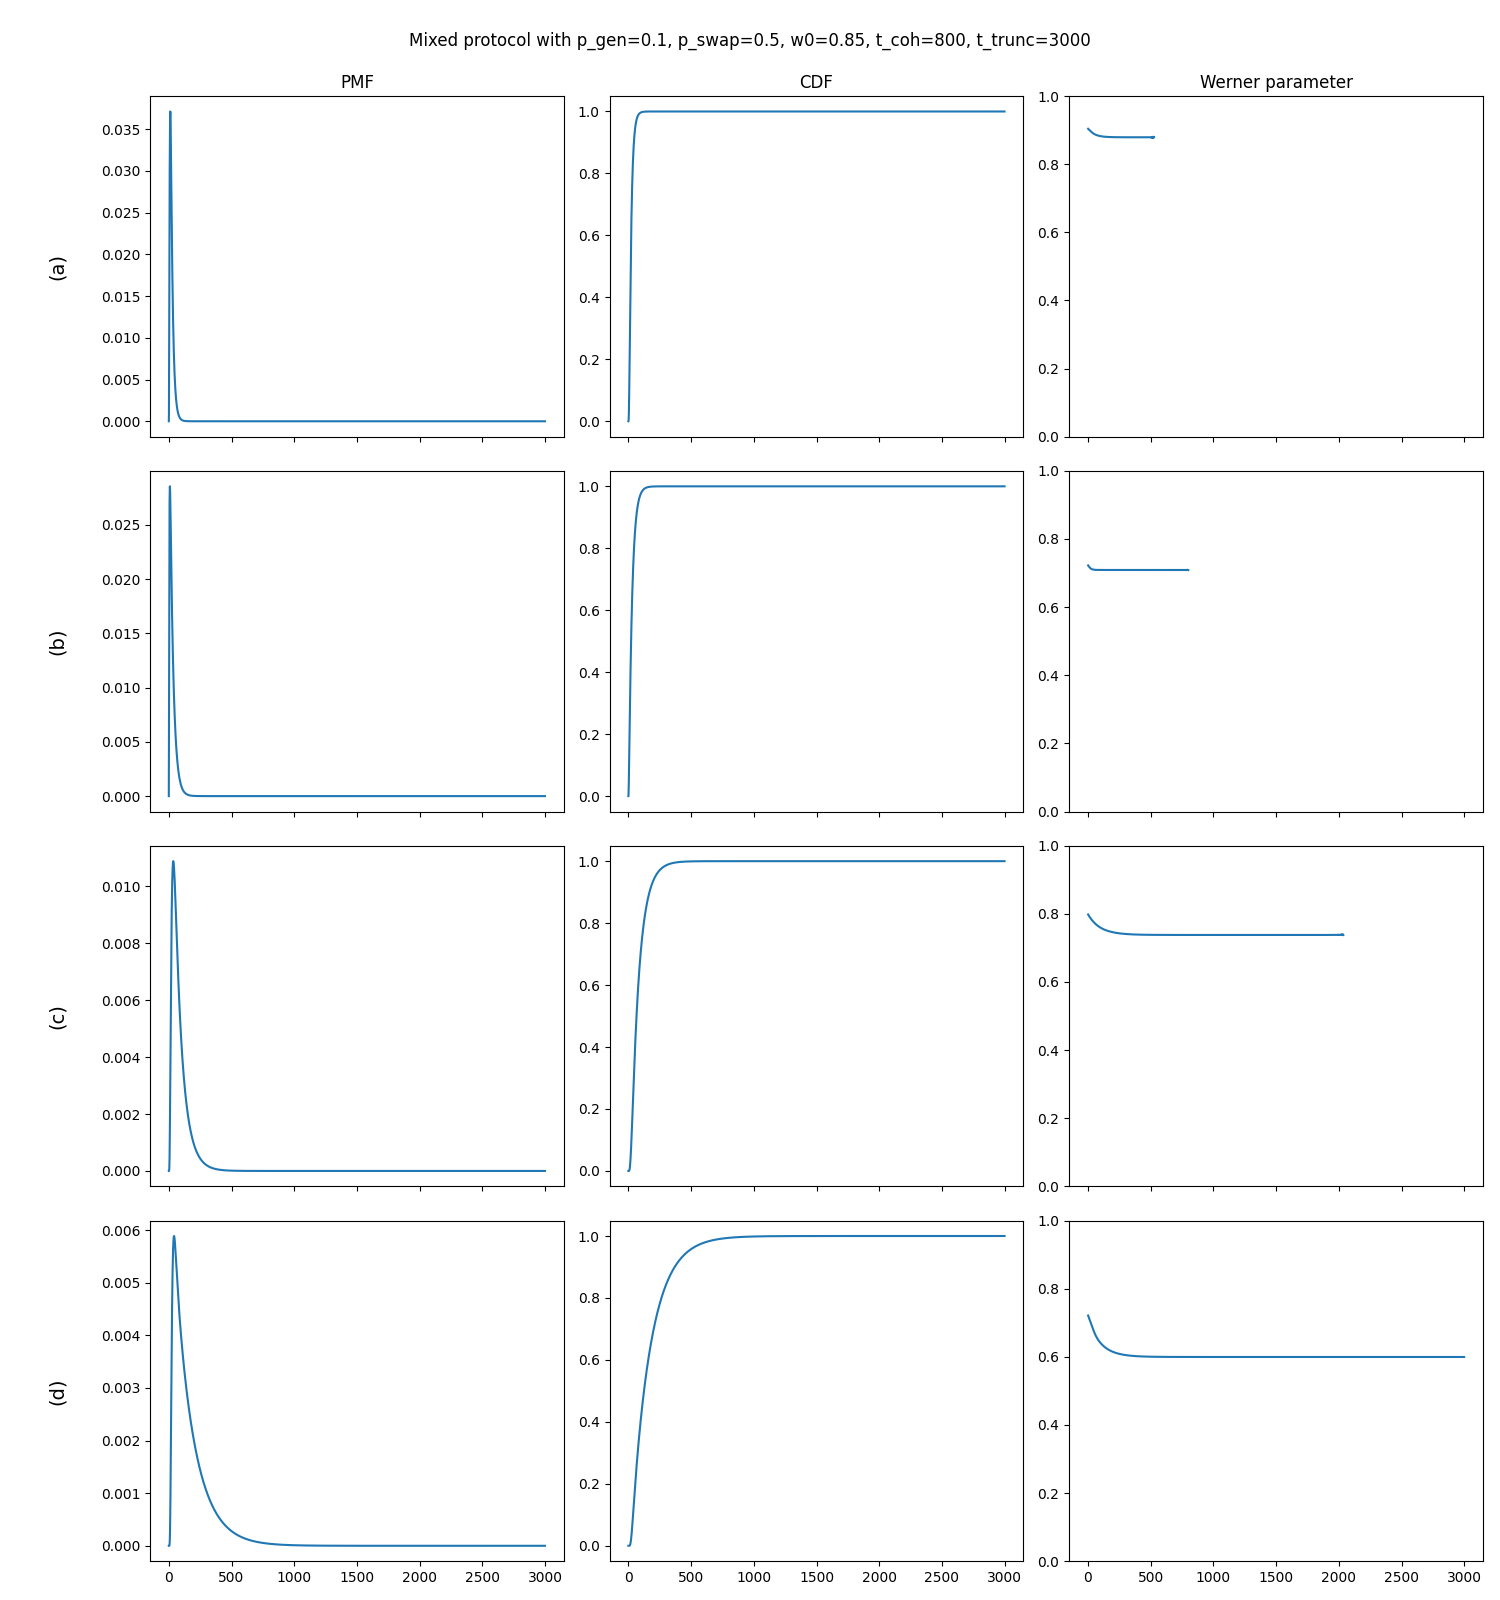
\includegraphics[width=0.8\linewidth]{images/mixed_protocol_no_cutoffs.png}
    \caption{These plots show the waiting time distribution and the Werner parameter for the mixed protocol described in Figure \ref{fig:mixed_protocol_sketch}. (a) After the generation of the elementary links and the distillation of 3 low-quality links $A-B$ into a high-quality one. (b) Consider $i \in {1,2,3}$. Three pair of links $(B_i-C_i, C_i-D_i)$, are swapped into the links $B_i-D_i$. (c) The three low-quality links $B_i-D_i$ are distilled into a single high-quality link $B-D$. (d) The end-link $A-D$ is produced starting from $A-B$ and $B-D$. The secret key rate at the end of the protocol is $3.1 * 10^{-3}$.} % todo: introduce secret key rate
    \label{fig:mixed_protocol} 
\end{figure}

We can get some general insights from the plots:
\begin{itemize}
    \item As the protocol units are applied, the probability that the link is produced at time $t$ shifts to a larger $t$, indicating longer waiting time.
    \item When protocol units different from distillation are applied, the Werner parameter decreases for most times $t$.
\end{itemize}

One important aspect to remark is that the Werner parameter curves are truncated if the corresponding PMF value goes under a certain threshold. This is because for these values of the PMF, the corresponding Werner parameter is unstable. % todo: define unstable

It is also interesting to notice that not always the distillation brings to higher values for the Werner parameter, like in this case.

In particular, the outcome of the Werner parameter depends on the quality of the input links, the times of their generation, and the time of decoherence $t_{coh}$. 
In the Figure \ref{fig:mixed_protocol_dist_comparison} we only consider the steps before and after distillation, presented as the second and third row in Figure \ref{fig:mixed_protocol}. We fix all the parameters except for the time of decoherence, that takes values $t_{coh} = {400, 1600}$.

\begin{figure}[ht]
    \centering
    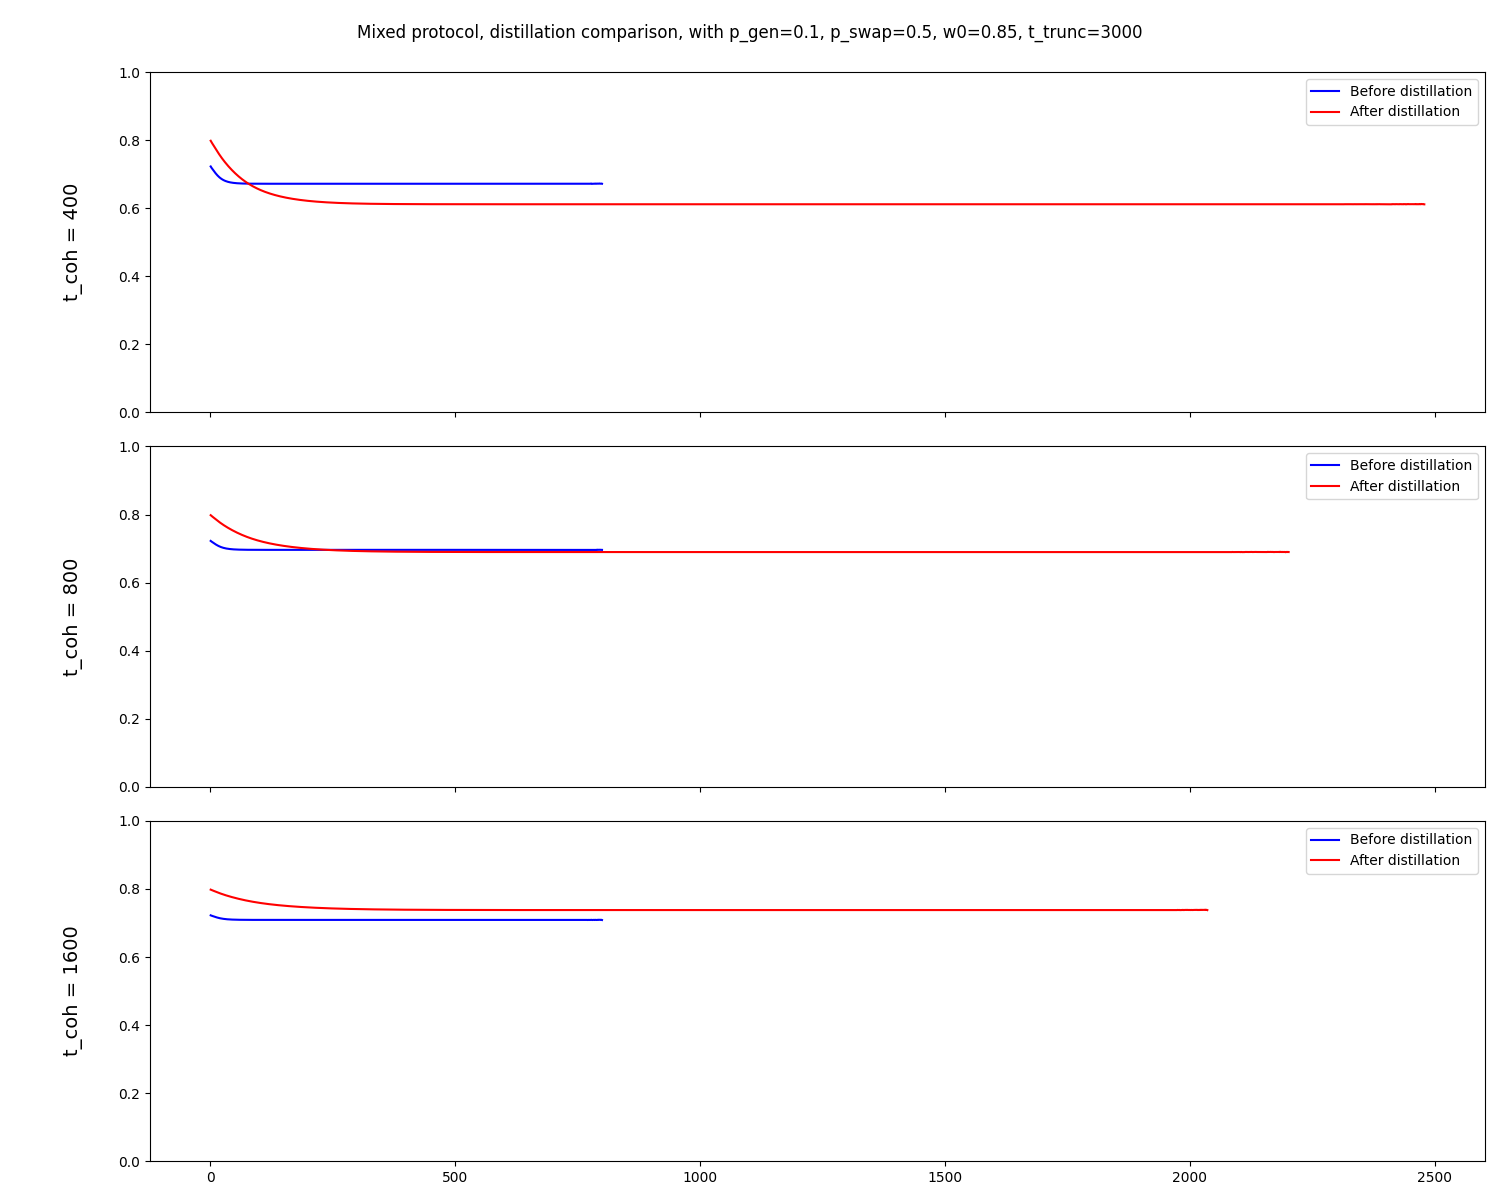
\includegraphics[width=1\linewidth]{images/mixed_protocol_dist_comp.png}
    \caption{}
    \label{fig:mixed_protocol_dist_comparison} 
\end{figure}

We notice that in one case the produced link has higher Werner parameter far all $t$, while in the other this is not true.

\newpage
\section*{Cutoffs}

The \textit{cutoff} operation selects the input links and accepts them if the cutoff condition is fulfilled. 

We define cutoffs condition and corresponding success probabilities $p_{\text{cut}}$ and Werner parameters $w_{out}$ in Table ??.
% todo: add table usign ai to convert image in latex

% Cutoffs are conditions imposed on the pair generated through \hyperref[section:heralded_entanglement_generation]{entanglement generation}. % is this true?

We consider only the case where cutoff \textbf{preceeds} by entanglement swapping or distillation; thus, the cutoff operation takes in input an entangled pair shared and give in ouput either:
\begin{itemize}
    \item the pair itself, if the cutoff condition is satisfied,
    \item nothing, if the condition is not satisfied.
\end{itemize} 

We model cutoffs together with these two protocols, by taking their described mathematical models and expanding them to include the cutoff conditions.


\subsection*{Waiting Time Distribution for Cutoffs}

We define a new binary variable $Y_{\text{cut}}$ representing whether the cutoff condition is fulfilled. 
In addition, we also define the waiting time of one cutoff attempt as $Z$, in contrast to $M$ for a swap or distillation attempt. 

We distinguish the waiting time of a successful and a failed attempt: 
\begin{itemize}
    \item In the case of success, we always have $Z_s = \max(T_A, T_B)$, i.e., we wait until two links are produced.
    \item In the case of failure, the waiting time $Z_f = t_{\text{fail}}(T_A, T_B)$ is different for different cutoff strategies. We have the following:
    \begin{itemize}
        \item for \textit{dif-time-cutoff}, $t_{\text{fail}}(T_A, T_B) = \min(T_A, T_B) + \tau$, because there is no need to wait for the second link longer than the cutoff threshold. 
        \item for \textit{max-time-cutoff}, $t_{\text{fail}}(T_A, T_B)$ is the constant $\tau$, i.e., the maximal allowed waiting time. 
        \item for \textit{fidelity-cutoff}, it is $t_{\text{fail}}(T_A, T_B) = \max(T_A, T_B)$.
    \end{itemize}
\end{itemize}

\paragraph*{Waiting Time for both pairs to be available}

A swap or distillation attempt followed by a cutoff, composed of several cutoff attempts. The expression for $M$ expressed in \ref{eq:waiting_time_pair} is now expressed as
\begin{equation}
    M = \sum_{k}\left\{\left[Y_{\text {cut }}^{(k)} \prod_{j=1}^{k-1}\left(1-Y_{\text {cut }}^{(j)}\right)\right] \cdot\left[Z_{\mathrm{s}}^{(k)}+\sum_{i=1}^{k-1}\left(Z_{\mathrm{f}}^{(i)}\right)\right]\right\} .    
\end{equation}

As a double check, if there is no cutoff ($Y_{\text {cut }}=1)$ we have that $k=1$ is the only surviving term and this expression coincide with \ref{eq:waiting_time_pair}.

\paragraph*{Separating Successful and Failure Attempts}

To calculate $\Pr(T_{out} = t)$, we need three joint distributions
\begin{enumerate}
    \item $P_f^{\prime}$ for unsuccessful input link preparation because of the cutoff,
    \item $P_{s, f}^{\prime}$ for successful preparation but unsuccessful swap/distillation,
    \item and $P_{s, s}^{\prime}$ for both successful.
\end{enumerate}

The prime notation indicates that they describe the waiting time of one attempt \textbf{with cutoff}, in contrast to one attempt in swap or distillation.

They are expressed as follows:
% \begin{aligned}
%     P_{\mathrm{f}}^{\prime}(t)= & \operatorname{Pr}\left(M=t, Y_{\mathrm{cut}}=0\right) \\
%     = & \sum_{t_{\mathrm{A}}, t_{\mathrm{B}}: t_{\mathrm{fail}}\left(t_{\mathrm{A}}, t_{\mathrm{B}}\right)+t_{\mathrm{c}}=t} \operatorname{Pr}\left(T_{\mathrm{A}}=t_{\mathrm{A}}, T_{\mathrm{B}}=t_{\mathrm{B}}\right) \\
%     & \cdot\left[1-p_{\mathrm{cut}}\right]\left(T_{\mathrm{A}}, T_{\mathrm{B}}\right) \\
%     P_{\mathrm{s}, \mathrm{f}}^{\prime}(t)= & \operatorname{Pr}\left(M=t, Y_{\mathrm{cut}}=1, Y=0\right) \\
%     = & \sum_{t_{\mathrm{A}}, t_{\mathrm{B}}: \max \left(t_{\mathrm{A}}, t_{\mathrm{B}}\right)+t_{\mathrm{c}}=t} \operatorname{Pr}\left(T_{\mathrm{A}}=t_{\mathrm{A}}, T_{\mathrm{B}}=t_{\mathrm{B}}\right) \\
%     & \cdot\left[p_{\mathrm{cut}} \cdot(1-p)\right]\left(t_{\mathrm{A}}, t_{\mathrm{B}}\right) \\
%     P_{\mathrm{s}, \mathrm{S}}^{\prime}(t)= & \operatorname{Pr}\left(M=t, Y_{\mathrm{cut}}=1, Y=1\right) \\
%     = & \sum_{t_{\mathrm{A}}, t_{\mathrm{B}}: \max \left(t_{\mathrm{A}}, t_{\mathrm{B}}\right)+t_{\mathrm{c}}=t} \operatorname{Pr}\left(T_{\mathrm{A}}=t_{\mathrm{A}}, T_{\mathrm{B}}=t_{\mathrm{B}}\right) \\
%     & \cdot\left[p_{\mathrm{cut}} \cdot p\right]\left(t_{\mathrm{A}}, t_{\mathrm{B}}\right)
% \end{aligned}


For \textbf{one attempt} in swap or distillation with cutoff, we then get
\begin{align}
    P_{s}(t) &= Pr(M=t, Y=1) = \sum_{k}\left[\binom{k-1}{j=1} P_{f}^{(j)} * P_{s, s}'\right](t), \\
    P_{f}(t) &= Pr(M=t, Y=0) = \sum_{k}\left[P_{f}^{(j)} * P_{s, f}'\right](t),
\end{align}
as well as the expressions in Fourier space analogous to
\begin{align}
    P_{s}(t) &= Pr(M=t, Y=1) = \mathcal{F}^{-1}\left[\frac{\mathcal{F}\left[P_{s, s}'\right]}{1-\mathcal{F}\left[P_{f}'\right]}\right], \\
    P_{f}(t) &= Pr(M=t, Y=0) = \mathcal{F}^{-1}\left[\frac{\mathcal{F}\left[P_{s, f}'\right]}{1-\mathcal{F}\left[P_{f}'\right]}\right].
\end{align}

The total waiting time then follows by substituting the expressions for $P_{f}$ and $P_{s}$ above in ?? and ??.

% For entanglement swap, i.e., constant success probability $p_{\text {swap, }}$, simplification can be made for this calculation. In this special case, $P_{\mathrm{s}, \mathrm{f}}^{\prime}$ and $P_{\mathrm{s}, \mathrm{S}}^{\prime}$ differ only by a constant and the same holds for $P_{\mathrm{s}}$ and $P_{\mathrm{f}}$.

\section*{Werner Parameter for Cutoffs}
For the Werner parameter, we now need three steps.

We start from calculating the resulting Werner parameter of a swap or distillation for the very last preparation attempt where $Y_{\text {cut }}=Y=1$. It is denoted by $W_{\mathrm{s}}^{\prime}$ and we only need to replace $P_{\mathrm{s}}$ by $P_{\mathrm{s}, \mathrm{S}}^{\prime}$ and $p \cdot w_{\text {out }}$ by $p_{\mathrm{cut}} \cdot p \cdot w_{\text {out }}$ in (12).

Next, we compute the Werner parameter $W_{\mathrm{s}}(t)$ as a function of time $t$ that includes the failed cutoff attempts, in ana$\log$ to the derivation of (13). $W_{\mathrm{s}}(t)$ is the Werner parameter that the pair of output links of cutofF will produce, given that the swap or distillation operation following is successful:

$$
W_{\mathrm{s}}(t)=\frac{\sum_{k=1}^{\infty}\left[\left(\begin{array}{c}
k-1 \\
* \\
j=1
\end{array} P_{\mathrm{f}}^{\prime}\right) *\left(P_{\mathrm{s}, \mathrm{s}}^{\prime} \cdot W_{\mathrm{s}}^{\prime}\right)\right](t)}{P_{\mathrm{s}}(t)}
$$

Finally, we consider the time consumed by failed attempts in SWAP or DIST and obtain

% $$
% W_{\text {out }}(t)=\frac{\sum_{k=1}^{\infty}\left[\binom{k-1}{\multirow{j=1}{*}{P_{\mathrm{f}}}} *\left(P_{\mathrm{S}} \cdot W_{\mathrm{s}}\right)\right](t)}{\operatorname{Pr}\left(T_{\text {out }}=t\right)}
% $$

Using the Fourier transform, the two expressions above become

$$
\begin{aligned}
W_{\mathrm{s}}(t) & =\mathcal{F}^{-1}\left[\frac{\mathcal{F}\left[P_{\mathrm{s}, \mathrm{s}}^{\prime} \cdot W_{\mathrm{s}}^{\prime}\right]}{1-\mathcal{F}\left[P_{\mathrm{f}}^{\prime}\right]}\right] \frac{1}{P_{\mathrm{s}}} \\
W_{\text {out }}(t) & =\mathcal{F}^{-1}\left[\frac{\mathcal{F}\left[P_{\mathrm{s}} \cdot W_{\mathrm{s}}\right]}{1-\mathcal{F}\left[P_{\mathrm{f}}\right]}\right] \frac{1}{\operatorname{Pr}\left(T_{\text {out }}=t\right)}
\end{aligned}
$$

\section*{Numerical Examples}

Here, we take the examples for the mixed protocol described in Figures \ref{fig:mixed_protocol_sketch} and \ref{fig:mixed_protocol} and add the cutoffs.

We consider the same parameters as before, with the addition of the cutoff strategy ...

Results for the waiting time and Werner parameter in the different stages are shown in Figure \ref{fig:mixed_protocol_cutoffs}.

\begin{figure}
    \centering
    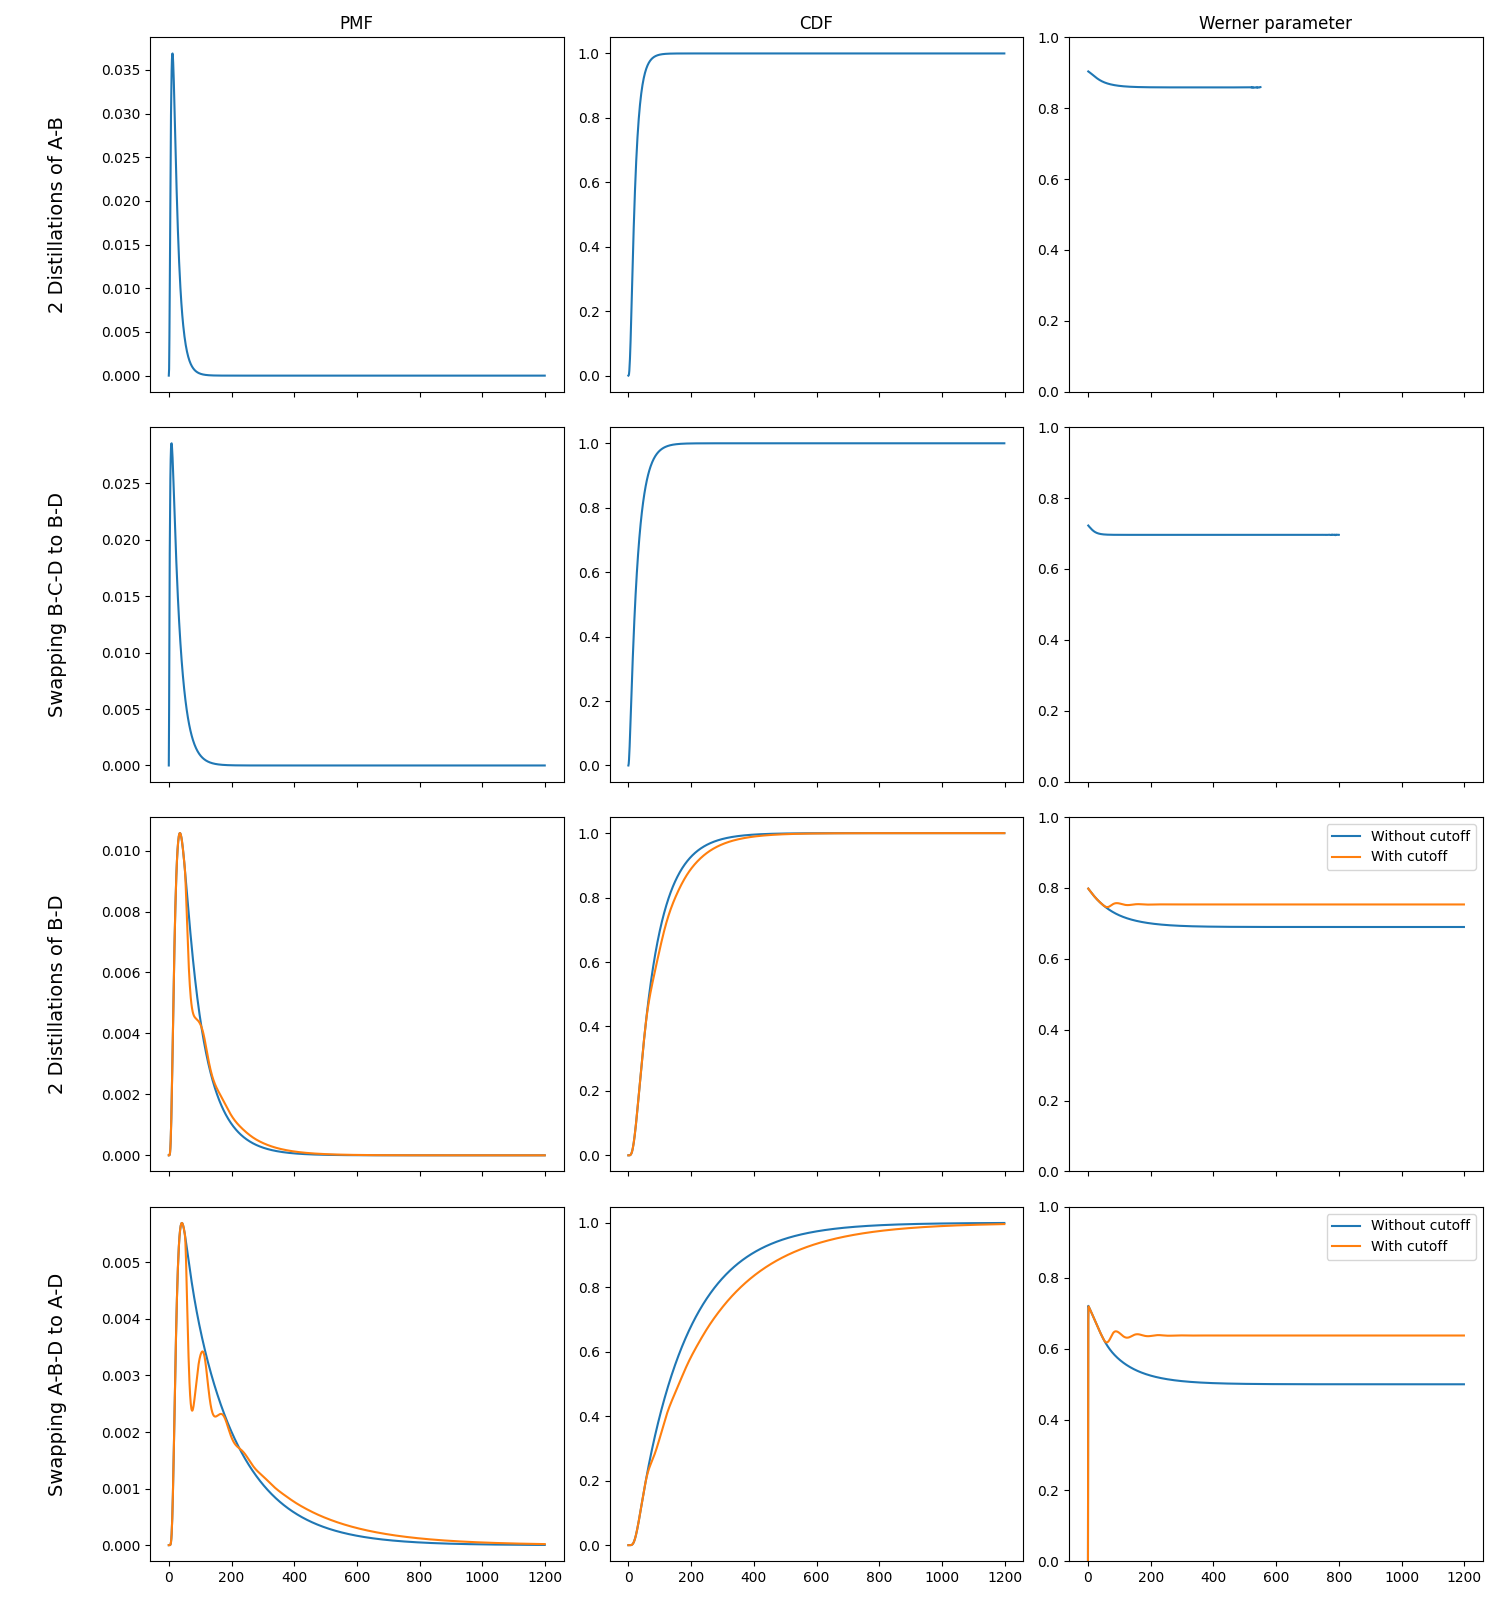
\includegraphics[width=1\linewidth]{images/mixed_protocol_cutoffs.png}
    \caption{(a)} 
    \label{fig:mixed_protocol_cutoffs}
\end{figure}

We can notice that ...
% talk also about secret key

% Results for the comparison for the Werner parameter before and after the distillation, with and without cutoffs, are shown in Figure \ref{fig:mixed_protocol_cutoffs_comparison}.

\section*{Closed Expressions in the Fourier Domain}

% todo: explain briefly the Fourier domain

% talk about discrete fourier transform

% todo: explain briefly the FFT and IFFT
- explain why the ft acts on a finite sequence of numbers

% todo: explain numpy fft and ifft
- what are the fft and ifft constraints?


\subsection*{Waiting Time Distribution for Entanglement Distillation}

Since the discrete Fourier transform acts on a finite sequence of numbers we first truncate the probability distribution at a fixed time $L$.

The Fourier transform is a linear map, converting convolutions into element-wise multiplication. As a consequence, taking the Fourier transform of both sides of Equation \ref{eq:waiting_time_distillation}, and then taking the inverse Fourier transform, yields
\begin{equation}\label{eq:waiting_time_distillation_fourier}
    \Pr(T_{\text{out}} = t) = \mathcal{F}^{-1} \left[ \frac{\mathcal{F}[P_s]}{1 - \mathcal{F}[P_f]} \right](t)
\end{equation}
which is a more elegant and efficient way to compute the waiting time distribution.

\paragraph*{Full Derivation}

The probability distribution of the total waiting time \( T_{\text{out}} \) for all attempts is given by Equation \ref{eq:waiting_time_distillation}, which we restate here for convenience:
\begin{equation}
    \Pr(T_{\text{out}} = t) = \sum_{k=1}^{\infty} \left[ \left(\ast_{j=1}^{k-1} P_f^{(j)} \right) \ast P_s \right](t) .
\end{equation}

Applying the Fourier transform \(\mathcal{F}\) to both sides, we get:
\begin{equation}
    \mathcal{F}[\Pr(T_{\text{out}} = t)] = \sum_{k=1}^{\infty} \left[ \left(\prod_{j=1}^{k-1} \mathcal{F}[P_f^{(j)}] \right) \cdot \mathcal{F}[P_s] \right](t)
\end{equation}

For $k$ attempts, the productory \(\prod_{j=1}^{k-1} \mathcal{F}[P_f^{(j)}]\) represents the convolution of the failure distributions in the Fourier domain. From the assumption made, these distributions \( P_f^{(j)} \) are identical copies (see Appendix \ref{paragraph:copies_of_a_random_variable}), so:
\begin{equation}
    \prod_{j=1}^{k-1} \mathcal{F}[P_f^{(j)}] = \left( \mathcal{F}[P_f] \right)^{k-1}
\end{equation}
which means that the equation simplifies to
\begin{equation}
    \mathcal{F}[\Pr(T_{\text{out}} = t)] = \sum_{k=1}^{\infty} \left( \left( \mathcal{F}[P_f] \right)^{k-1} \cdot \mathcal{F}[P_s] \right) .
\end{equation}

Using the identity for the sum of a geometric series \(\sum_{k=1}^{\infty} x^{k-1} = \frac{1}{1-x}\), we can state that
\begin{equation}
    \sum_{k=1}^{\infty} \left( \mathcal{F}[P_f] \right)^{k-1} = \frac{1}{1 - \mathcal{F}[P_f]}
\end{equation}
thus, incorporating the success term \(\mathcal{F}[P_s]\), we get:
\begin{equation}
\mathcal{F}[\Pr(T_{\text{out}} = t)] = \frac{\mathcal{F}[P_s]}{1 - \mathcal{F}[P_f]}
\end{equation}

Finally, applying the inverse Fourier transform \(\mathcal{F}^{-1}\), we obtain:
\begin{equation}
    \Pr(T_{\text{out}} = t) = \mathcal{F}^{-1} \left[ \frac{\mathcal{F}[P_s]}{1 - \mathcal{F}[P_f]} \right](t)
\end{equation}

\subsection*{Werner Parameter for Entanglement Distillation}

The transformation of Equation \ref{eq:werner_parameter_distillation} to Fourier space involves the same concepts and yields
\begin{equation}\label{eq:werner_parameter_distillation_fourier}
    W_{\text{out}} = \mathcal{F}^{-1} \left[ \frac{\mathcal{F}[P_s \cdot W_s]}{1 - \mathcal{F}[P_f]} \right] \frac{1}{\Pr(T_{out}=t)}(t) .
\end{equation}

Again, the convolution has become a productory of identical copies of the same random variable; the resulting term, exponentiated to $k-1$, is then transformed through geometric series, yielding the final expression.

\subsection*{Entanglement Swapping in the Fourier Domain}

Equations \ref{eq:waiting_time_swap} and \ref{werner_parameter_swap} can also be moved to the Fourier space as follows.
Both expressions can be written in Fourier space by substituting $P_s = p_{swap} \cdot m(t)$ and $P_f = (1 - p_{swap}) \cdot m(t)$ in the Equations for entanglement distillation \ref{eq:waiting_time_distillation_fourier} and \ref{eq:werner_parameter_distillation_fourier}, yielding
\begin{equation}
    \Pr(T_{\text{out}} = t) = \mathcal{F}^{-1} \left[ \frac{\mathcal{F}[p_{swap} \cdot m(t)]}{1 - \mathcal{F}[(1 - p_{swap}) \cdot m(t)]} \right](t)
\end{equation}
and
\begin{equation}
    W_{\text{out}} = \mathcal{F}^{-1} \left[ \frac{\mathcal{F}[p_{swap} \cdot m(t) \cdot W_s]}{1 - \mathcal{F}[(1 - p_{swap}) \cdot m(t)]} \right] \frac{1}{\Pr(T_{out}=t)}(t)
\end{equation}
where $m$ is defined in Equation \ref{eq:pdf_waiting_time_pair_convolution}.

\subsection*{Cutoffs in the Fourier Domain}
% derivation

\appendix

\chapter*{Mathematical Background} % todo: when merging, divide math. background for q.mechanics and for q.repeaters

\section*{Convolution}

Convolution is a fundamental mathematical operation used to combine two functions to produce a third function, which represents how the shape of one function is modified by the other. 

For two discrete functions \(a\) and \(b\), the convolution \(a * b\) is defined as:

\begin{equation}
    (a * b)(z) = \sum_{x=0}^{z} a(x) \cdot b(z - x)
\end{equation}

\paragraph*{Convolution of two Probability Distributions}
In the context of probability distributions, if \(X\) and \(Y\) are independent random variables with probability distribution functions \(p_X\) and \(p_Y\), their sum \(Z = X + Y\) has a probability distribution function \(p_Z\) given by the convolution of \(p_X\) and \(p_Y\):
\begin{equation}\label{eq:convolution}
    p_Z(z) = \sum_{x=0}^{z} p_X(x) \cdot p_Y(z - x)
\end{equation}

Thus, convolution is used to determine the probability distribution of the sum of independent random variables by combining their individual probability distributions.

\paragraph*{Example} 

Consider this simple example. Let $X$ and $Y$ discrete independent random variables. 

The probability distribution $\Pr(Z = z)$ of the random variable $Z = X + Y$ is computed as follows:
\begin{equation*}\label{eq:convolution_example}
    \begin{array}{|c|c|c|c|c|c|c|}
        \hline
        x & \Pr(X = x) & y & \Pr(Y = y) & z & \Pr(Z = z) & \text{Derivation of }\Pr(Z = z)\\
        \hline
        0 & 0.2 & 0 & 0.3 & 0 & 0.06 & 0.2 \cdot 0.3 \\
        \hline
        1 & 0.5 & 1 & 0.4 & 1 & 0.23 & 0.2 \cdot 0.4 + 0.5 \cdot 0.3 \\
        \hline
        2 & 0.3 & 2 & 0.3 & 2 & 0.35 & 0.2 \cdot 0.3 + 0.5 \cdot 0.4 + 0.3 \cdot 0.3 \\
        \hline
         &  &  &  & 3 & 0.27 & 0.5 \cdot 0.3 + 0.3 \cdot 0.4 \\
        \hline
         &  &  &  & 4 & 0.09 & 0.3 \cdot 0.3 \\
        \hline
    \end{array}
\end{equation*}

Note that $\Pr(Z = z)$ has five elements (all the possible sums), and it is valid as its probabilities sum to 1.

\paragraph*{Associativity}
\begin{samepage}
    The convolution operator \( * \) is associative, meaning that for any three functions \(a\), \(b\), and \(c\):
    \begin{equation}\label{eq:convolution_associativity} 
        (a * b) * c = a * (b * c)
    \end{equation}        
\end{samepage}

\section*{Random Variables}

In this section, we fix notation on random variables and operations on them. 

Most random variables in the context of quantum repeaters
\begin{itemize}
    \item are discrete,
    \item have as domain a subset of nonnegative integers.
\end{itemize}

\paragraph*{PDF}\label{paragraph:pdf}
Let $X$ be such a random variable, then its probability distribution function is a map
\begin{equation}
    p_X : x \mapsto \Pr(X = x)
\end{equation} 
which describes the probability that its outcome will be $x \in \{0, 1, 2, \ldots \}$.

\paragraph*{CDF}\label{paragraph:cdf}
Equivalently, $X$ is described by its cumulative distribution function
\begin{equation}
    \Pr(X \leq x) = \sum_{y=0}^{x} \Pr(X = y),
\end{equation}

which is transformed to the probability distribution function as 
\begin{equation}
    \Pr(X = x) = \Pr(X \leq x) - \Pr(X \leq x - 1).
\end{equation}

\paragraph*{Independent Random Variables}\label{paragraph:independent_random_variables}
Two random variables $X$ and $Y$ are independent if 
\begin{equation}
    \Pr(X = x \text{ and } Y = y) = \Pr(X = x) \cdot \Pr(Y = y)
\end{equation}
for all $x$ and $y$ in the domain.

\paragraph{Copies of a Random Variable}\label{paragraph:copies_of_a_random_variable} By a \textit{copy} of $X$, we mean a fresh random variable which is independent from $X$ and identically distributed (i.i.d.).
We will denote a copy by a superscript in parentheses. For example, $X^{(1)}$, $X^{(142)}$ and $X^{(A)}$ are all copies of $X$.

\paragraph*{Expected Value}
The mean of $X$ is denoted by 
\begin{equation}\label{eq:expectation}
    E[X] = \sum_{x=0}^{\infty} \Pr(X = x) \cdot x
\end{equation}

and can equivalently be computed as 
\begin{equation}
    E[X] = \sum_{x=1}^{\infty} \Pr(X \geq x).
\end{equation}

\paragraph*{Function of Random Variables}\label{paragraph:function_of_random_variables}
If $f$ is a function which takes two nonnegative integers as input, then the random variable $f(X, Y)$ has probability distribution function defined as

\begin{equation}
    \Pr(f(X, Y) = z) := \sum_{\substack{x=0, y=0 \\ f(x,y)=z}}^{\infty} \Pr(X = x \text{ and } Y = y).
\end{equation}

\paragraph*{Sum of Random Variables}\label{paragraph:sum_of_random_variables}
An example of such a function is addition. 

Define $Z := X+Y$ where $X$ and $Y$ are independent, then the probability distribution $p_Z$ of $Z$ is given by 
\begin{equation}
    p_Z(z) = \Pr(Z = z) = \sum_{\substack{x=0, y=0 \\ x+y=z}}^{\infty} \Pr(X = x \text{ and } Y = y).
\end{equation}

But since $y = z - x$, this is equivalent to
\begin{align}
    p_Z(z) = \Pr(Z = z) &= \sum_{\substack{x=0}}^{z} \Pr(X = x \text{ and } Y = z - x) \\ 
                        &= \sum_{\substack{x=0}}^{z} \Pr(X = x) \cdot Pr(Y = z - x) \\
                        &= \sum_{x=0}^{z} p_X(x) \cdot p_Y (z - x)
\end{align}
which is the convolution of the distributions $p_X$ and $p_Y$ (see \ref{eq:convolution}), denoted as $p_Z = p_X * p_Y$.

Notice that, since the convolution operator $*$ is associative (see \ref{eq:convolution_associativity}), writing $a * b * c$ is well-defined, for functions $a$, $b$, $c$, from the nonnegative integers to the real numbers.

In general, \textbf{the probability distribution of sums of independent random variables equals the convolutions of their individual probability distribution functions}.

\section*{Geometric Distribution}\label{section:geometric_distribution}

The geometric distribution is a discrete probability distribution that models the number of trials needed to achieve the first success in a sequence of independent Bernoulli trials, each with the same success probability $p$.

\subsection*{Probability Distribution Function (PDF)}\label{subsection:geometric_pdf}

The probability distribution function (PDF) of a geometric distribution gives the probability that the first success occurs on the $t$-th trial. It is defined as:
\begin{equation}
    \Pr(T = t) = p \cdot (1 - p)^{t-1} \quad \text{for} \quad t \in \{1, 2, 3, \ldots \},
\end{equation}
where:
\begin{itemize}
    \item $T$ is the random variable representing the trial number of the first success,
    \item $p$ is the probability of success on each trial,
    \item $(1 - p)$ is the probability of failure on each trial.
\end{itemize}

This formula expresses that the first $t-1$ trials must be failures, each occurring with probability $(1-p)$, and the $t$-th trial must be a success (with probability $p$).

\subsection*{Cumulative Distribution Function (CDF)}\label{subsection:geometric_cdf}

The cumulative distribution function (CDF) of a geometric distribution gives the probability that the first success occurs on or before the $t$-th trial. It is defined as:
\begin{equation}
    \Pr(T \leq t) = 1 - (1 - p)^t.
\end{equation}

\paragraph*{Derivation of the CDF}
The CDF of a geometric distribution can be derived from its PDF as follows:
\begin{align*}
    \Pr(T \leq t) &= 1 - \Pr(T > t) \\
    &= 1 - \sum_{k=t+1} \Pr(T = k) \\
    &= 1 - \left\{p (1 - p)^t + p (1 - p)^{t+1} + p (1 - p)^{t+2} + \ldots\right\} \\
    &= 1 - p (1 - p)^t \sum_{k=0} (1 - p)^k \\
    &= 1 - (1 - p)^t \sum_{k=0} p (1 - p)^k \\
    &= 1 - (1 - p)^t.
\end{align*} % tocheck

\chapter*{A Numerical Example}

This appendix contains a numerical example of the protocols described. We consider the following parameters:
\begin{itemize}
    \item the probability of success for entanglement generation is $p_{\text{gen}} = 0.5$,
    \item the probability of success for entanglement swapping is $p_{\text{dist}} = 0.5$,
    \item the initial Werner parameter of the generated links is $w_{\text{gen}} = 0.9$,
\end{itemize}
and assume that the system is not subjected to decoherence ($t_{coh} = \infty$).

\section*{Entanglement Generation}

The probability distribution of the waiting time for entanglement generation is a geometric distribution (see Appendix \ref{section:geometric_distribution}) with $p = 0.5$, shown in Figure \ref{fig:gen_waiting_time}.
\begin{figure}[ht]
    \centering
    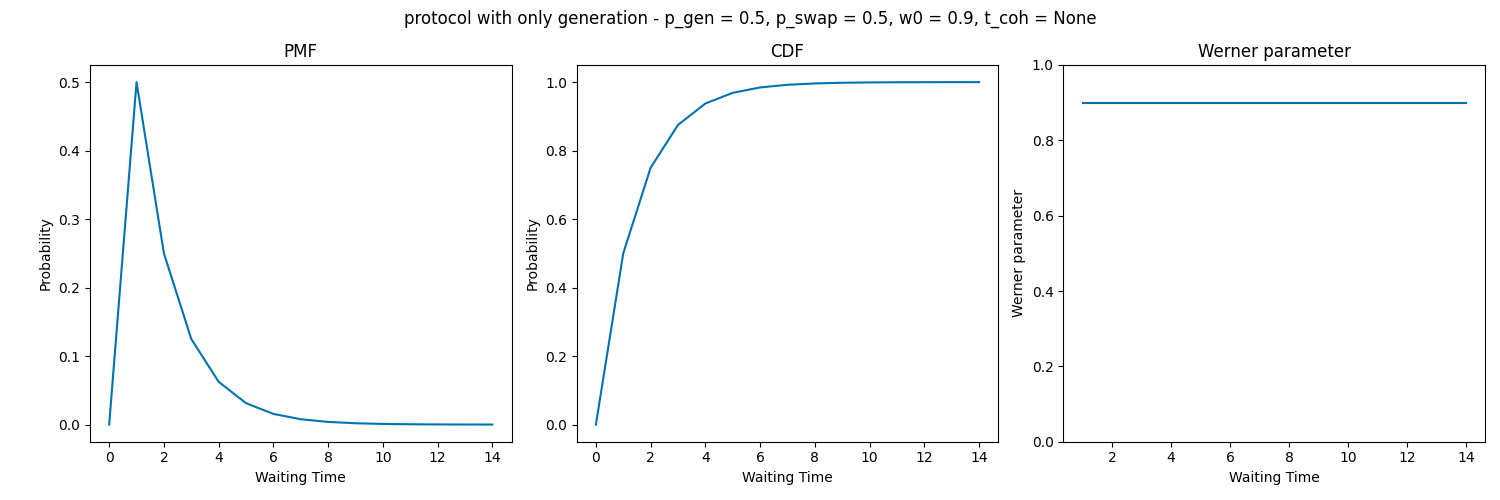
\includegraphics[width=1\linewidth]{images/dist_tests/only generation.png}
    \caption{Plots for entanglement generation. The PMF is a geometric distribution governed by $p_{gen} = 0.5$; for such high value, the CDF reaches a value close to 1 in few time steps. The Werner parameter is costant.}
    \label{fig:gen_waiting_time}
\end{figure}

In the table below, we show the probability distribution of the waiting time for entanglement generation, as well as the corresponding output average Werner parameter, for some selected times.

\begin{equation*}
    \begin{array}{|c|c|c|c|}
        \hline
        \text{Time Step} & \text{PMF} & \text{CDF} & \text{Werner} \\
        \hline
        t = 1 & 0.50000 & 0.50000 & 0.90000 \\
        \hline
        t = 2 & 0.25000 & 0.75000 & 0.90000 \\
        \hline
        t = 3 & 0.12500 & 0.87500 & 0.90000 \\
        \hline
        t = 10 & 0.00098 & 0.99902 & 0.90000 \\
        \hline
        t = 50 & 0.00000 & 1.00000 & 0.90000 \\
        \hline
    \end{array}
    \label{tab:gen_waiting_time}
\end{equation*}

In this particular example, as $p_{gen} = (1 - p_{gen}) = 0.5$, The probability of achieving a link at time $t = i$ is $(0.5)^i$.

For entanglement generation, for all $t$, the average Werner parameter is the constant $w_0 = 0.9$. As a matter of fact, indipendently from the number of attempts needed to achieve a link, its quality will always be the same.

\section*{Entanglement Distillation}

The probability distribution of the waiting time for entanglement distillation is shown in Figure \ref{fig:dist_waiting_time}.

\begin{figure}[ht]
    \centering
    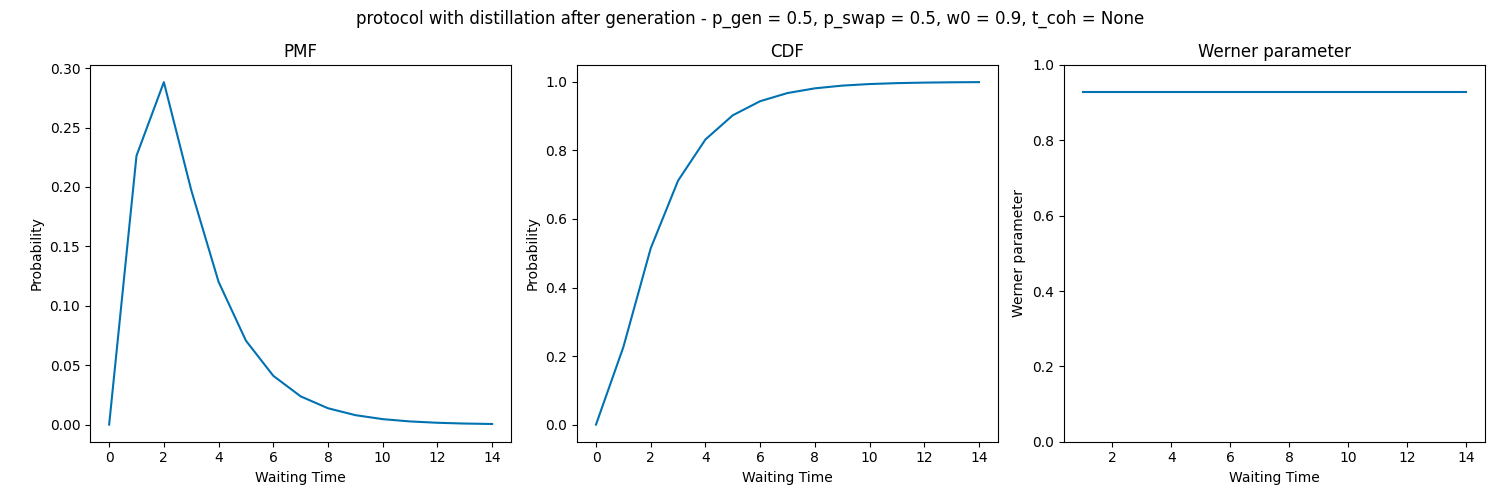
\includegraphics[width=1\linewidth]{images/dist_tests/distillation after generation.png}
    \caption{Plots for entanglement distillation, after generation. The CDF for the waiting time, for all the values of $t$, is shifted to the right with respect to Figure \ref{fig:gen_waiting_time} of entanglement generation only. This indicates longer waiting times. The Werner parameter is again costant, as no decoherence is considered in this example.}
    \label{fig:dist_waiting_time}
\end{figure}

In the table below, we show, for some selected times, the PDF, the CDF, and the corresponding Werner parameter for the waiting time of entanglement distillation.

\begin{equation*}
    \begin{array}{|c|c|c|c|}
        \hline
        \text{Time Step} & \text{PMF} & \text{CDF} & \text{Werner} \\
        \hline
        t = 1 & 0.22625 & 0.22625 & 0.92818 \\
        \hline
        t = 2 & 0.28819 & 0.51444 & 0.92818 \\
        \hline
        t = 3 & 0.19739 & 0.71183 & 0.92818 \\
        \hline
        t = 10 & 0.00460 & 0.99370 & 0.92818 \\
        \hline
        t = 50 & 0.00000 & 1.00000 & 0.92819 \\
        \hline
    \end{array}
\end{equation*}

In the following, we show the calculations for $t={1,2}$ rows.

\paragraph*{Probability Distribution Function}

Here, we show the computation of the probability distribution function $\Pr(T_{\text{d}} = t)$ for the waiting time of entanglement distillation, for some selected times.

For $t = 1$, we consider the case when the distillation suceeds immediately. Hence we take into consideration only the random variable $P_s$: to achieve the distilled link at time $t=1$, the protocol has to succeeds at its first attempt: 
\begin{equation}
    \Pr(T_{\text{d}} = 1) = P_s(t = 1) = 0.5 \cdot 0.5 \cdot 0.905 = 0.22625
\end{equation}
where we plugged $t = 1$ in the Equation \ref{eq:waiting_time_success_failure} for one successful attempt of distillation.

For $t = 2$, we have to consider both failure and success random variables described in Equation \ref{eq:waiting_time_success_failure}, which are then used in Equation \ref{eq:waiting_time_distillation}. Plugging $t=2$, and expanding the equation for clarity, we get 
\begin{equation}\label{eq:distillation_t2}
    \Pr(T_{\text{d}} = 2) = P_s(2) + (P_f \ast P_s)(2) + (P_f \ast P_f \ast P_s)(2) + \ldots
\end{equation}
where we have theoretically an infinite number of terms, truncated in practical calculations.

We compute the values for a success and a failure at time $t=2$ expanding the sum in Equation \ref{eq:waiting_time_success_failure}
\begin{align}
    P_s(2) &= \left(0.25 \cdot 0.5 \cdot 0.905\right) + \left(0.5 \cdot 0.25 \cdot 0.905\right) + \left(0.25 \cdot 0.25 \cdot 0.905\right) = \\
           &= 0.25 \cdot \left(0.5 + 0.5 + 0.25 \right) \cdot 0.905 = 0.28281 \\
    P_f(2) &= 0.25 \left(0.5 + 0.5 + 0.25\right) \cdot 0.095 = 0.02968
\end{align}
where we considered all the contributions given by both links succeding at times $t={1,2}$, as the distillation starts when both input links are generated.

To consider distillation success after failure we compute $[P_s \ast P_f](2)$. To do that \textbf{we need to convolve the PDFs of $P_s$ and $P_f$} (see Appendix \ref{eq:convolution}):
\begin{equation*}
    \begin{array}{|c|c|c|c|c|}
        \hline
        t & P_s(t) & P_f(t) & [P_s \ast P_f](t) & [P_f \ast P_s \ast P_f](t) \\
        \hline
        0 & 0 & 0 & 0 & 0 \\
        \hline
        1 & 0.22625 & 0.02375 & 0 & 0 \\
        \hline
        2 & 0.28281 & 0.02968 & 5.3734 \cdot 10^{-3} & 0 \\
        \hline
    \end{array}
\end{equation*}
where we computed $[P_s \ast P_f](2)$ according to Equation \ref{eq:convolution}:
\begin{equation}
    [P_s * P_f](2) = 0 + 0.22625 \cdot 0.02325 + 0 = 5.3734 \cdot 10^{-3} .
\end{equation}

Thus, the probability distribution function for $t = 2$ is, according to Equation \ref{eq:distillation_t2}:
\begin{equation}
    \Pr(T_{\text{d}} = 2) = 0.28281 + 0.00537 = 0.28819
\end{equation}
where we disregarded the higher order terms, as they are all zero.

\paragraph*{Werner Parameter}

We first compute the probability of success for the distillation operation, which is given by
\begin{equation}
    p_d = \frac{1 + w_A w_B}{2} = \frac{1+2w_0}{2}
\end{equation}
and is equal to
\begin{equation}
    p_d = (1 + 0.81) / 2 = 0.905 .
\end{equation}

The Werner parameter for the output links of the distillation operation is given by
\begin{equation}
    w_d = \frac{w_A + w_B + 4 w_A \cdot w_B}{6 p_d} = \frac{2w_0 + 4w_0^2}{6 p_d}
\end{equation}
and is equal to
\begin{equation}
    w_d = 0.92818 .
\end{equation}

Since we are not considering decoherence in this example, the average ouput Werner parameter of the distilled link is constant for all $t$.

\section*{Two-Level Entanglement Distillation}

Now, on top of the entanglement distillation, we add a second level of distillation. The probability distribution of the waiting time for this two-level entanglement distillation $\Pr(T_{dd} = t)$ is shown in Figure \ref{fig:two_level_distillation_waiting_time}.

\begin{figure}[ht]
    \centering
    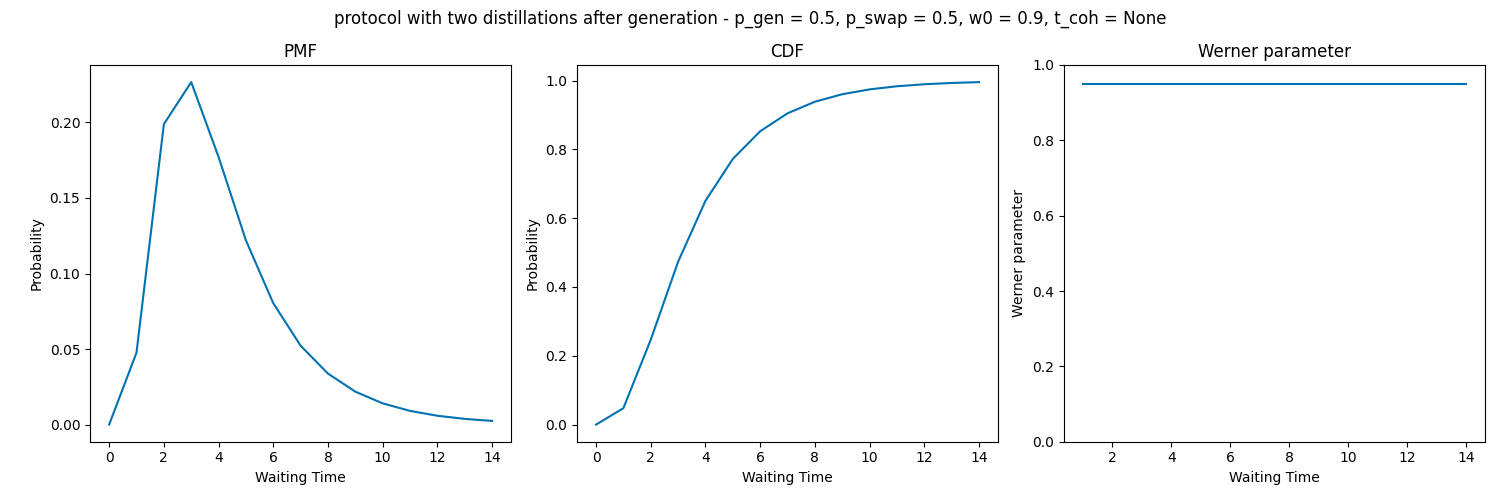
\includegraphics[width=1\linewidth]{images/dist_tests/two distillations after generation.png}
    \caption{The probability distribution of the waiting time for two-level entanglement distillation.}
    \label{fig:two_level_distillation_waiting_time}
\end{figure}

In the table below, we show, for some selected times, the PDF, the CDF, and the corresponding Werner parameter for this protocol.
\begin{equation*}
    \begin{array}{|c|c|c|c|}
        \hline
        \text{Time Step} & \text{PMF} & \text{CDF} & \text{Werner} \\
        \hline
        t = 1 & 0.04764 & 0.04764 & 0.94948 \\
        \hline
        t = 2 & 0.19884 & 0.24649 & 0.94948 \\
        \hline
        t = 3 & 0.22670 & 0.47319 & 0.94948 \\
        \hline
        t = 10 & 0.01406 & 0.97442 & 0.94948 \\
        \hline
        t = 50 & 0.00000 & 1.00000 & 0.94948 \\
        \hline
    \end{array}
\end{equation*}

\paragraph*{Probability Distribution Function}

For $t = 1$, we have again the edge case for which we consider only an attempt succeeding at time $t=1$, without failures  
\begin{equation}
    \Pr(T_{dd} = 1) = P_s'(1) = 0.22625 \cdot 0.93075 = 0.04764 
\end{equation}
where we used the prime notation to differentiate this from the previous case. 

For $t = 2$,
\begin{equation}
    \Pr(T_{dd} = 2) = P_s'(2) + (P_f' \ast P_s')(2) + (P_f' \ast P_f' \ast P_s')(2) + \ldots
\end{equation}
is computed as before, and yields
\begin{equation}
    \Pr(T_{dd} = 2) = 0.19884 .
\end{equation}

\paragraph*{Werner Parameter}

The probability of success for the two-level distillation operation is
\begin{equation}
    p_{dd} = \frac{1 + w_A w_B}{2} = \frac{1 + w_d^2}{2} = 0.93075 .
\end{equation}

The Werner parameter for the output links of the two-level distillation operation is given by
\begin{equation}
    w_{dd} = \frac{w_A + w_B + 4 w_A \cdot w_B}{6 p_{dd}} = \frac{2 w_d + 4 w_d^2}{6 p_{dd}} = 0.94974
\end{equation}
and, again, it is constant for all the times $t$ as no decoherence is considered.

\section*{Entanglement Swapping}

The probability distribution of the waiting time for entanglement swapping is shown in Figure \ref{fig:swap_waiting_time}.
\begin{figure}[ht]
    \centering
    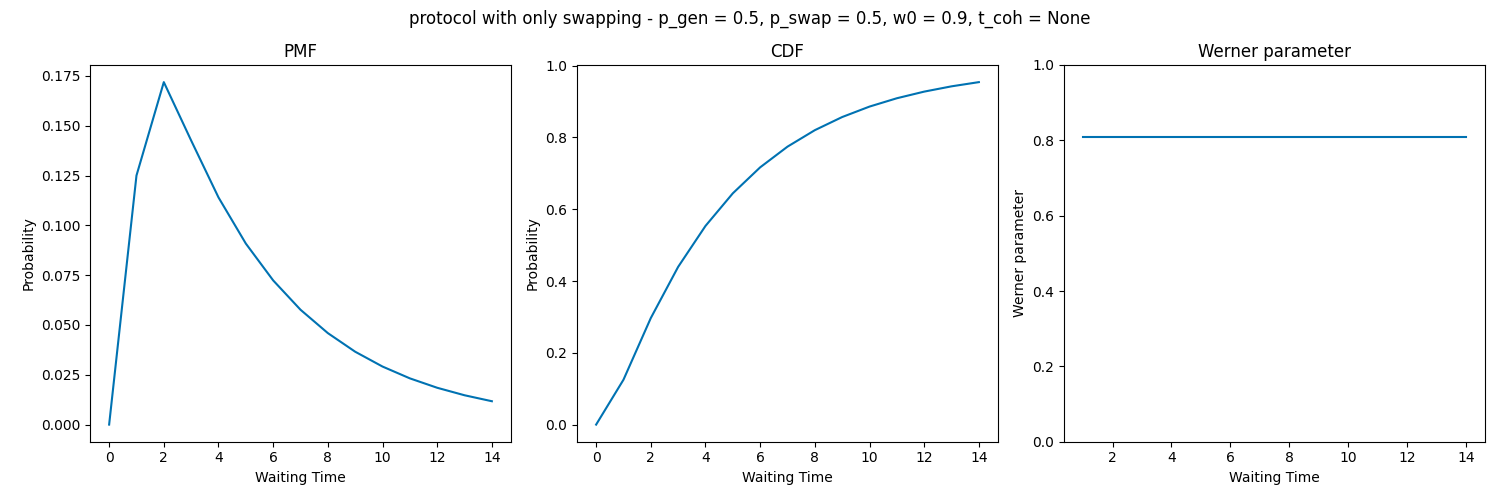
\includegraphics[width=1\linewidth]{images/dist_tests/only swapping.png}
    \caption{The probability distribution of the waiting time for entanglement swapping.}
    \label{fig:swap_waiting_time}
\end{figure}

In the table below, we show, for some selected times, the PDF, the CDF, and the corresponding Werner parameter for the waiting time of entanglement swapping.
\begin{equation*}
    \begin{array}{|c|c|c|c|}
        \hline
        \text{Time Step} & \text{PMF} & \text{CDF} & \text{Werner} \\
        \hline
        t = 1 & 0.12500 & 0.12500 & 0.81000 \\
        \hline
        t = 2 & 0.17188 & 0.29688 & 0.81000 \\
        \hline
        t = 3 & 0.14258 & 0.43945 & 0.81000 \\
        \hline
        t = 10 & 0.02913 & 0.88595 & 0.81000 \\
        \hline
        t = 50 & 0.00000 & 0.99999 & 0.81000 \\
        \hline
    \end{array}
\end{equation*}

\end{document}
